\documentclass[a4paper,headsepline=3pt,headinclude=true,12pt,oneside]{scrbook}
\usepackage[left=2cm,right=2cm,top=1cm,bottom=3cm,includeheadfoot]{geometry}
\usepackage{scrlayer-scrpage}
\usepackage{mwe}
\usepackage[origlayout=true,automark,colors={ph}]{URpagestyles}
\usepackage{lipsum} %fuer Fuelltexte

\usepackage{iftex}%automatische Auswahl des richtigen Fontloaders und der Eingabekodierung
%Es liefert das Makro \ifPDFTeX. Die Abfragen können entfernt werden, wenn nur eine bestimmte Variante verwendet wird.
\ifPDFTeX%falls mit pdfLaTeX kompiliert wird
	\usepackage[utf8]{inputenc}
	\usepackage[T1]{fontenc}
	\usepackage[ngerman]{babel} 
	%\usepackage[english]{babel} %Sparache aendern
\else%falls mit Lua oder XeLaTeX kompiliert wird
	\usepackage{fontspec}
	\usepackage{polyglossia}
	\setmainlanguage{german} 
	%\setmainlanguage{english} %Sprache aendern 
\fi
\usepackage{lmodern} %moderne Schriftarten
\usepackage{csquotes}
\usepackage{titletoc} %partielles Inhaltsverzeichnis

%alles mit Tabellen
\usepackage{array}
\usepackage{booktabs}
\usepackage{longtable}
\usepackage{csvsimple}
\usepackage{multirow}
\usepackage{makecell}

%\usepackage[dvipsnames]{xcolor} %Farben, optionen fuer mehr Voreinstellungen
%aufpassen beim Drucken, Drucker sind fast alle schlecht kalibriert, erst eine Testseite drucken

\usepackage{xspace} %Abstaende
\usepackage{setspace} %Zeilenabstand

%alles mit Bildern
\usepackage{float}
\usepackage{placeins}
\usepackage{graphicx}
\usepackage{caption}
\usepackage{subcaption}
\usepackage{sidecap}
\usepackage{wrapfig}
\usepackage{pdfpages}

%alles mit Mathematik
\DeclareMathSizes{18}{18}{18}{18}
\usepackage{upgreek}
\usepackage{paralist}
\usepackage{amsmath}
\usepackage{amssymb}
\usepackage{amscd}
\usepackage[output-decimal-marker={,}]{siunitx}
\usepackage{thmtools}
\usepackage{pgfplots}
\pgfplotsset{compat=1.16}

%code texen
\usepackage{listings}
\lstset{ %Beispielkonfiguration fuer C-code
  backgroundcolor=\color{lightgray!50!white},   % choose the background color; you must add \usepackage{color} or \usepackage{xcolor}; should come as last argument
  basicstyle=\footnotesize,        % the size of the fonts that are used for the code
  breakatwhitespace=false,         % sets if automatic breaks should only happen at whitespace
  breaklines=true,                 % sets automatic line breaking
  captionpos=b,                    % sets the caption-position to bottom
  commentstyle=\color{orange},     % comment style
  deletekeywords={sizeof},         % if you want to delete keywords from the given language
  extendedchars=true,              % lets you use non-ASCII characters; for 8-bits encodings only, does not work with UTF-8
  firstnumber=1,                   % start line enumeration with line 1000
  frame=single,                    % adds a frame around the code
  keepspaces=true,                 % keeps spaces in text, useful for keeping indentation of code (possibly needs columns=flexible)
  %keywordstyle=\color{red!50!black},% keyword style
  keywordstyle=\color{blue},% keyword style
  language=C++,                    % the language of the code
  morekeywords={__constant__, __shared__, __device__, __host__, __global__, __managed__, float2, float3, float4, dim3, int2, int3, int4, uint, half, cudaStream_t, cudaEvent_t, cudaError_t, cudnnError_t, cusparseError_t, cublasError_t, curandError_t, cufftError_t, cusolverError_t, __kernel, kernel, __constant, constant, __local, local, __private, private, __global, global, cl_device_id, cl_platform_id, cl_int, cl_uint, cl_float, cl_double, string, cl_mem, cl_kernel, size_t, cl_event, cl_program, cl_context, cl_command_queue, FILE, restrict, event_t, ptrdiff_t , intptr_t, uintptr_t, device_ptr, device_vector, host_vector, vector, Platform, Context, CommandQueue, Buffer, Program, Kernel, Sources, Device, cl_context_properties, hipStream_t, cufftHandle, cufftComplex, cufftReal, cufftDouble, cufftDoubleComplex, clfftSetupData, clfftDim, fftw_complex, fftw_plan, curandStateSobol32_t, curandStateScrambledSobol32_t, curandStateSobol64_t, curandStateScrambledSobol64_t, curandState (XORWOW), curandStatePhilox4_32_10_t, curandStateMRG32k3a, curandStateMtgp32_t, curandGenerator_t, curandState, clrngMrg31k3pHostStream, clrngMrg31k3pStream, clprobdistExponential, clqmcLatticeRule, clqmcLatticeRuleStream, cublasHandle_t, cublasOperation_t, cuComplex, cuDoubleComplex, clsparseIdx_t, cldenseVector, clsparseCreateResult, clsparseCreateSolverResult, clsparseCsrMatrix, cusolverDnHandle_t, cusolverSpHandle_t, cusolverRfHandle_t, magma_queue_t, magma_int_t, LocalVector, CG, LocalStencil, __attribute__, aligned_allocator, auto, tensorflow, trt, tf, keras, Mat, cudnnHandle_t, cudnnTensorDescriptor_t, cudnnFilterDescriptor_t, cudnnConvolutionDescriptor_t, cudnnConvolutionFwdAlgo_t, ncclComm_t, MPI_INT},% if you want to add more keywords to the set
  numbers=left,                    % where to put the line-numbers; possible values are (none, left, right)
  numbersep=5pt,                   % how far the line-numbers are from the code
  numberstyle=\small\color{black}, % the style that is used for the line-numbers
  rulecolor=\color{black},         % if not set, the frame-color may be changed on line-breaks within not-black text (e.g. comments (green here))
  showspaces=false,                % show spaces everywhere adding particular underscores; it overrides 'showstringspaces'
  showstringspaces=false,          % underline spaces within strings only
  showtabs=false,                  % show tabs within strings adding particular underscores
  stepnumber=2,                    % the step between two line-numbers. If it's 1, each line will be numbered
  stringstyle=\color{green!50!black}, % string literal style
  identifierstyle=\color{black},
  tabsize=2,	                   % sets default tabsize to 2 spaces
  title=\lstname                   % show the filename of files included with \lstinputlisting; also try caption instead of title
}
\expandafter\ifx\csname li\endcsname\relax
\let\li=\lstinline
\else\errmessage{li schon definiert \meaning\li}%
\fi

%Literaturverzeichnis
\usepackage[backend=biber, citestyle=numeric, bibstyle=numeric]{biblatex}
\addbibresource{lit.bib} %richtigen Pfad ersetzen

%Index
\usepackage{makeidx}
\makeindex

\setlength{\parindent}{0pt} %keine Absatzeinzüge
\setlength{\parskip}{\baselineskip}

%Links
\usepackage[colorlinks=true,
            linkcolor=black,
            urlcolor=gray,
            citecolor=gray,
            bookmarks=true]{hyperref}
\usepackage{tabularx} %Tabellencounter, nach hyperref
\usepackage[toc,nopostdot]{glossaries} %Glossar, nach hyperref
\makeglossaries
\newglossaryentry{API}
{
	name=API,
	description={application programming interface, Programmierschnittstelle.},
	plural=APIs
}

\newglossaryentry{Arbeit}
{
	name=Arbeit,
	description={typischerweise eine Zahl von Flops, ein Maß für die Lesitung, die ein Programm erbringen muss.},
	plural=Arbeiten
}

\newglossaryentry{arithmetische Intensität}
{
	name=arithmetische Intensität,
	description={Verhältnis von Arbeit zum Datenverkehr.},
	plural=arithmetische Intensitäten
}

\newglossaryentry{Block}
{
	name=Block,
	description={ein evtl. mehrdimensionaler Verbund von Threads in Software (CUDA). Jeder Block besteht aus der gleichen Anzahl an Threads.},
	plural=Blöcke
}

\newglossaryentry{compute capability}
{
	name=compute capability,
	description={eine Versionsnummer der Chiparchitektur, die u.A. bestimmt, welche Features von CUDA auf der GPU implementiert wurden.},
	plural=compute capabilitys
}

\newglossaryentry{Command Queue}
{
	name=Command Queue,
	description={eine Menge von Instruktionen, die der Reihe nach abgehandelt werden sollen (OpenCL).},
	plural=Command Queues
}

\newglossaryentry{constant Memory}
{
	name=constant Memory,
	description={siehe erstes Vorkommen},
	plural=constant Memorys
}

\newglossaryentry{Datenverkehr}
{
	name=Datenverkehr,
	description={eine Zahl an Bytes, die während des Ausführens eines Programms insgesamt transferriert wird.}
}

\newglossaryentry{Gang}
{
	name=Gang,
	description={ein evtl. mehrdimensionaler Verbund von Vectors in Software (OpenACC). Jede Gang besteht aus der gleichen Anzahl an Vectors.},
	plural=Gangs
}

\newglossaryentry{global Memory}
{
	name=global Memory,
	description={siehe erstes Vorkommen},
	plural=global Memorys
}

\newglossaryentry{Grid}
{
	name=Grid,
	description={die Gesamtheit aller Blöcke (Nvidia).},
	plural=Grids
}

\newglossaryentry{Halfwarp}
{
	name=Halfwarp,
	description={ein Verbund von 16 Threads in Hardware (Nvidia, CUDA Terminologie).},
	plural=Halfwarps
}

\newglossaryentry{Handle}
{
	name=Handle,
	description={ein eindeutiger Referenzwert zu einer vom Betriebssystem verwalteten Systemressource.},
	plural=Handles
}

\newglossaryentry{Kernel}
{
	name=Kernel,
	description={eine kleine Recheneinheit, die auf die GPU ausgelagert werden soll.},
	plural=Kernel
}

\newglossaryentry{Kontext}
{
	name=Kontext,
	description={ein Handle für das OpenCL Programm (Speicherobjekte, Programs, Command Queues, ...).},
	plural=Kontexte
}

\newglossaryentry{local Memory}
{
	name=local Memory,
	description={Speicher (cached) eines einzelnen Threads (CUDA). \\ ein kleiner, sehr schneller Speicher, den sich alle Workitems einer Workgroup teilen (OpenCL). Pro SM wird einer verbaut (Nvidia).},
	plural=local Memorys
}

\newglossaryentry{MTIU}
{
	name=MTIU,
	description={Multi Threaded Instruction Unit, ein kleiner Controller, der Instruktionen an die Warps ausgibt.},
	plural=MTIUs
}

\newglossaryentry{nvcc}
{
	name=nvcc,
	description={Nvidia C(++) Compiler}
}

\newglossaryentry{nvlink}
{
	name=nvlink,
	description={eine High-Speed Datenschnittstelle für Nvidia Grafikkarten in Clustern.}
}

\newglossaryentry{NVPTX}
{
	name=NVPTX,
	description={Nvidia Parallel Thread Execution, eine assemblerartige Sprache, in die nvcc Devicecode übersetzt.}
}

\newglossaryentry{page-locked Memory}
{
	name=page-locked Memory,
	description={allozierter Speicher, der nicht vom Betriebssystem verschoben werden darf.}
}

\newglossaryentry{parallele Effizienz}
{
	name=parallele Effizienz,
	description={Verhältnis von Speedup zur Anzahl der eingesetzten Prozessoren.},
	plural=parallele Effizienzen
}

\newglossaryentry{PCIe}
{
	name=PCIe,
	description={Peripheral Component Interconnect Express, die standard-Schnittstelle für Steckkarten.}
}

\newglossaryentry{Peak Bandwidth}
{
	name=Peak Bandwidth,
	description={maximale interne Speicherbandbreite.},
	plural=Peak Bandwidth
}

\newglossaryentry{Peak Performance}
{
	name=Peak Performance,
	description={maximale Performance eines Prozessors.},
	plural=Peak Performances
}

\newglossaryentry{Performance}
{
	name=Performance,
	description={das Verhältnis von Flops zur benötigten Rechenzeit, ein Maß für die Effizienz von Soft- und Hardware.},
	plural=Performances
}

\newglossaryentry{Platform}
{
	name=Platform,
	description={eine OpenCL Imolementierung in Software.},
	plural=Platformen
}

\newglossaryentry{private Memory}
{
	name=private Memory,
	description={Speicher (cached) eines einzelnen Workitems (OpenCL).},
	plural=private Memorys
}

\newglossaryentry{shared Memory}
{
	name=shared Memory,
	description={siehe erstes Vorkommen},
	plural=shared Memorys
}

\newglossaryentry{SM}
{
	name=SM,
	description={Streaming Multiprocessor, Eine Recheneinheit bestehend aus mehreren Warps, einer MTIU und shared memory.},
	plural=SMs
}

\newglossaryentry{Speedup}
{
	name=Speedup,
	description={Faktor, um den ein paralleles Programm schneller läuft, als die sequentielle Variante.},
	plural=Speedups
}

\newglossaryentry{Stream}
{
	name=Stream,
	description={eine Menge von Instruktionen, die der Reihe nach abgehandelt werden sollen (CUDA).},
	plural=Streams
}

\newglossaryentry{texture Memory}
{
	name=Texture Memory,
	description={siehe erstes Vorkommen},
	plural=Texture Memorys
}

\newglossaryentry{Thread}
{
	name=Thread,
	description={die kleinste Recheneinheit einer GPU in CUDA, in Hardware auf Nvidia GPUs auch CUDA Core genannt.},
	plural=Threads
}

\newglossaryentry{Vector}
{
	name=Vector,
	description={die kleinste Recheneinheit einer GPU in OpenACC.},
	plural=Vectors
}

\newglossaryentry{Warp}
{
	name=Warp,
	description={Kombination zweier Halfwarps.},
	plural=Warps
}

\newglossaryentry{Wavefront}
{
	name=Wavefront,
	description={ein Verbund von 32 oder 64 Workitems in Hardware (AMD).},
	plural=Wavefronts
}

\newglossaryentry{Worker}
{
	name=Wavefront,
	description={ein Verbund von 32 Vectors in Hardware (Nvidia, OpenACC Terminologie).},
	plural=Workers
}

\newglossaryentry{Workgroup}
{
	name=Workgroup,
	description={ein evtl. mehrdimensionaler Verbund von Workitems in Software (OpenCL). Jede Workgroup besteht aus der gleichen Anzahl an Workitems.},
	plural=Workgroups
}

\newglossaryentry{Workitem}
{
	name=Workitem,
	description={die kleinste Recheneinheit einer GPU in OpenCL.},
	plural=Workitems
}
 %Glossardefinitionen einfuegen, richtigen Pfad ersetzen

\DeclareCaptionFont{black}{\color{black}}
\DeclareCaptionFormat{listing}{
  \colorbox[rgb]{1,1,1}{
    \parbox{\textwidth}{\hspace{15pt}#1#2#3}
  }
}
\captionsetup[lstlisting]{format=listing, labelfont=black, textfont=black, singlelinecheck=false, margin=0pt, font={bf,footnotesize}}

\renewcommand*{\familydefault}{\sfdefault}
\newcommand*{\pck}[1]{\texttt{#1}}
\newcommand*{\code}[1]{\texttt{#1}}
\newcommand*{\repl}[1]{\textrm{\textit{#1}}}
\newcommand{\cmd}[1]{\par\medskip\noindent\fbox{\ttfamily#1}\par\medskip\noindent}
\setcounter{secnumdepth}{\sectionnumdepth}
\newsavebox{\remarkbox}
\sbox{\remarkbox}{\emph{Anmerkung:~}}
\newcounter{iterator}
\usepackage{colortbl}

%meta Informationen
\author{Thomas Karl}
\title{Wissenschaftliches Rechnen auf Grafikkarten}
\subtitle{Universit\"at Regensburg}
\date{Sommersemester 2020}
\renewcommand{\titlepagestyle}{URtitle} 
\renewcommand{\lstlistingname}{Codebeispiel}
%\renewcommand{\thechapter}{\Roman{chapter}}
%\renewcommand{\thesection}{\thechapter~\arabic{section}}

\cfoot*{ }
\ofoot*{\thepage}% the pagenumber in the center of the foot, also on plain pages
\ihead*{ }% Name and title beneath each other in the inner part of the foot
\ohead*{\headmark}
\automark[subsection]{section}

\newcommand*\Laplace{\mathop{}\!\mathbin\bigtriangleup}

\begin{document}
\begin{onehalfspacing}
	\pagenumbering{Roman} %Die ersten Seiten roemisch nummeriert	

	%\maketitle
	
	
\includepdf{titlepage.pdf}	
	\newpage
	
	\tableofcontents
	\newpage
	
	\listoffigures
	\addcontentsline{toc}{chapter}{\listfigurename}
	\newpage
	
	\listoftables
	\addcontentsline{toc}{chapter}{\listtablename}
	\newpage
    
	\renewcommand{\lstlistlistingname}{Liste der Codebeispiele} %Listenname umbenennen
    \lstlistoflistings
    \addcontentsline{toc}{chapter}{\lstlistlistingname}
    \newpage
%    
    \printglossaries %Glossar automatisch im Inhaltsverzeichnis

%%%%%%%%%%%%%%%%%%%%%%%%%%%%%%%%%%%%%%%%%%%%%%%%%%%%%%%%%%%%%%%
%%%%%%%%%%%%%%%%%%%% eigentlicher Inhalt %%%%%%%%%%%%%%%%%%%%%% 
	\pagenumbering{arabic} %ab jetzt arabisch nummeriert
	\setcounter{page}{1} %beginnend mit eins, pdf-reader einstellen mit bookmarks=true in den Optionen von hyperref

    \startcontents[Einführung in High-Performance-Computing]
    \printcontents[Einführung in High-Performance-Computing]{l}{1}{\chapter*{Einführung in High-Performance-Computing}\setcounter{tocdepth}{2}}
    	\chapter{Einf\"uhrung in High-Performance-Computing} 
		\section{Amdahl's Law}
		Gegeben sei ein sequentielles Programm. Zerlegt man dieses in Teile, die theoretisch parallelisierbar sind, und jene, die in jedem Fall sequentiell laufen müssen, so ergibt sich die Gesamtlaufzeit $T$ als Summe 
		\begin{equation}\label{eq1:am}
		    T = t_p + t_s
        	\end{equation}
        	
        	wobei $t_p$ die Laufzeit des parallelisierbaren Anteils und $t_s$ die des sequentiellen bezeichnet. Zu den unparallelisierbaren Anteilen zählen typischerweise Prozessinitialisierung oder Speicherverwaltung. Benutzt man ferner Hardware zum Ausführen des Programms, auf der insgesamt $n_P$ Prozessoren oder Prozessorkerne dauerhaft zur Verfügung stehen, so gilt für den sogenannten maximalen Speedup $S$:
		\begin{equation}
		    S = \frac{T}{t_s + \frac{t_p}{n_p}} \leq \frac{T}{t_s} = \frac{T}{T-t_p}
        	\end{equation}	   
		
		Dabei wird das Verhältnis $\varepsilon = \frac{S}{n_P}$ auch als \gls{parallele Effizienz} bezeichnet. Als \Gls{Speedup} wird der Faktor bezeichnet, um den sich die Geschwindigkeit eines parallelen Programms gegenüber der sequentielle Vatiante verbessert. Abbildung \ref{1:am} zeigt diesen Speedup in Abhängigkeit von $n_p$ für verschiedene Verhältnisse von $\frac{t_p}{T}$.
		Allerdings hängt der sequentielle Anteil auch von der Parallelisierung selbst ab. Durch z.B. Prozessorkommunikation oder Synchronisation entsteht in der Gesamtlaufzeit ein zusätzlicher Summand	$t_{O(n_P)}$. In diesem Beispiel steigt der Anteil linear mit $n_P$. Dies ist jedoch nicht zwingend der Fall. Damit ergibt sich der maximale \Gls{Speedup}:		
		\begin{equation}
		    S = \frac{T}{t_s + t_{O(n_P)} + \frac{t_p}{n_p}} \leq \frac{T}{t_s} = \frac{T}{T-t_p}		
		\end{equation}
		
		Diese Kurve konvergiert nun nicht mehr gegen $\frac{T}{t_s}$, sondern erreicht ein Maximum, um danach wieder abzufallen (Abb. \ref{1:am_prax}). In der Praxis ergibt sich ein Optimum, eine Anzahl von Prozessoren, bei der sich der maximale \Gls{Speedup} erzielen lässt. Eine Vergrößerung dieser Anzahl hat einen negativen Effekt, da der Geschwindigkeitsgewinn durch die weiteren Prozessoren den Aufwand der Prozessorkommunikation nicht mehr kompensiert.


		\section{Gustafson's Law}
		Amdahl stellte mit seinem Gesetz eine worst-case Abschätzung auf, bei der sich die Laufzeit mit der Zahl der Prozessoren linear verbessern lässt. Amdahl geht dabei von einer festen Problemgröße aus. Gustafsons Gesetz hingegen geht von einem festen Zeitfenster aus. In diesem wächst die Problemgröße mit Anzahl der Prozessoren. Mit dieser Zahl wächst linear auch die Größe der Aufgabe, die unter den Voraussetzungen gelöst werden kann.

		Setzt man $P=t_p/T$ lässt sich \ref{eq1:am} umschreiben:
		\begin{equation}
			1 = (1 - P) + P
		\end{equation}
		
		Lässt sich der parallele Anteil unter Vernachlässigung von $t_{O(n_P)}$ gleichzeitig auf $n_P$ Prozessoren ausführen, so gilt für den \Gls{Speedup}:
    		\begin{equation}
        		S(n_P) = (1 - P) + n_P P
    		\end{equation}
		
		Der parallele Anteil wächst also linear mit der Anzahl der Prozessoren. Im Gegensatz zu Amdahl wird der sequentielle Anteil mit zunehmenden $n_p$ bedutungslos, wirkt also nicht beschränkend.
		 
		\section{Amdahl vs. Gustafson}		
		Nach Amdahl ist die \gls{parallele Effizienz}:
        	\begin{equation}
           	\varepsilon_{\text{Amdahl}}(n_P)    = \frac1{n_P}\cdot \frac1{(1-P)+P/n_P} = \frac1{n_P(1-P)+P}
        	\end{equation}
        	
        	Nach Gustafson ist die \gls{parallele Effizienz}:
		\begin{equation}
			\varepsilon_{\text{Gustafson}}(n_P) = 1 - \frac{n_P-1}{n_P}\cdot (1-P) = P +\frac{1-P}{n_P}
		\end{equation}
		
		Laut Amdahl geht die \gls{parallele Effizienz} im Limit einer großen Prozessorzahl immer gegen null, bei Gustafson existiert eine untere Schranke $P$:
		\begin{gather*}
			\lim\limits_{n_P \rightarrow \infty}\varepsilon_{\text{Amdahl}}(n_P)    = 0 \\        
			\lim\limits_{n_P \rightarrow \infty}\varepsilon_{\text{Gustafson}}(n_P) = P
		\end{gather*}
		
		Welches Modell nun Anwendung finden sollte, hängt von der Problemstellung ab. Gustafsons Gesetz sollte auf Probleme angewandt werden, falls sich die Promblemgrö\ss e auf die Parallelisierung anpassen lässt, andernfalls Amdahl. In jedem Fall geben Amdahl und Gustafson eine Ober- und Untergrenze für den \Gls{Speedup} an. 
        
		\begin{figure}[h]
		\centering
    		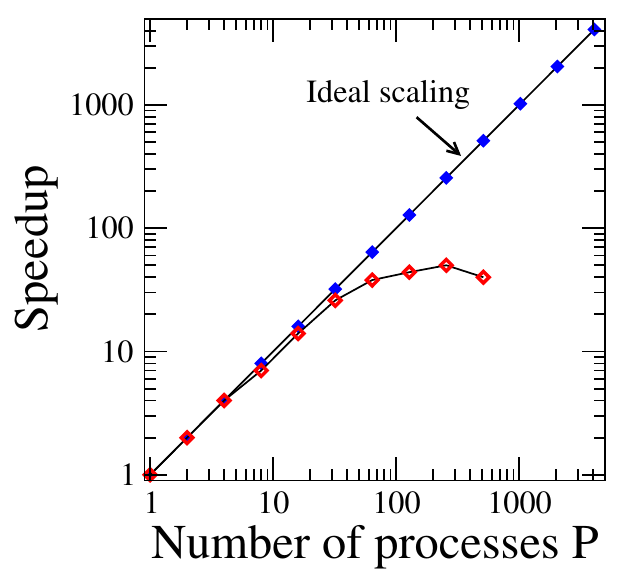
\includegraphics[height=0.4\textwidth]{chapter1/pictures/Amdahl_praxis.png}
    		\caption[Speedup laut Amdahl mit Prozesskommunikation]{Der Speedup laut Amdahl bei einer bestimmten Zahl an Prozessoren unter Berücksichtigung von Prozessorkommunikation. Ab einer bestimmten Anzahl nimmt der Speedup wieder ab. (doppelt-logarithmische Skala) \autocite{carch}}
    		\label{1:am_prax}
		\end{figure}
        
		\newpage
		\begin{figure}[h]
		\centering
    		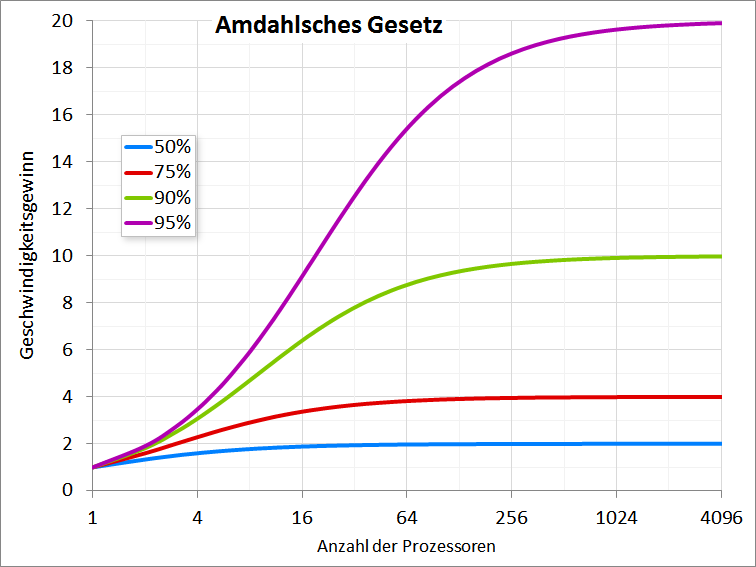
\includegraphics[height=0.5\textwidth]{chapter1/pictures/Amdahl.png}
    		\caption[Speedup laut Amdahl ohne Prozesskommunikation]{Der Speedup laut Amdahl bei einer bestimmten Zahl an Prozessoren ohne Berücksichtigung von Prozesskommunikation für verschiedene Verhältnisse von $t_s/T$. Der Speedup konvergiert schnell gegen $T/t_s$. (einfach-logarithmische Skala) \autocite{wikiAmdahl}}
    		\label{1:am}
		\end{figure}
		
		\newpage
		\section{Roofline Model}
		\begin{figure}[t]
		\centering
	    	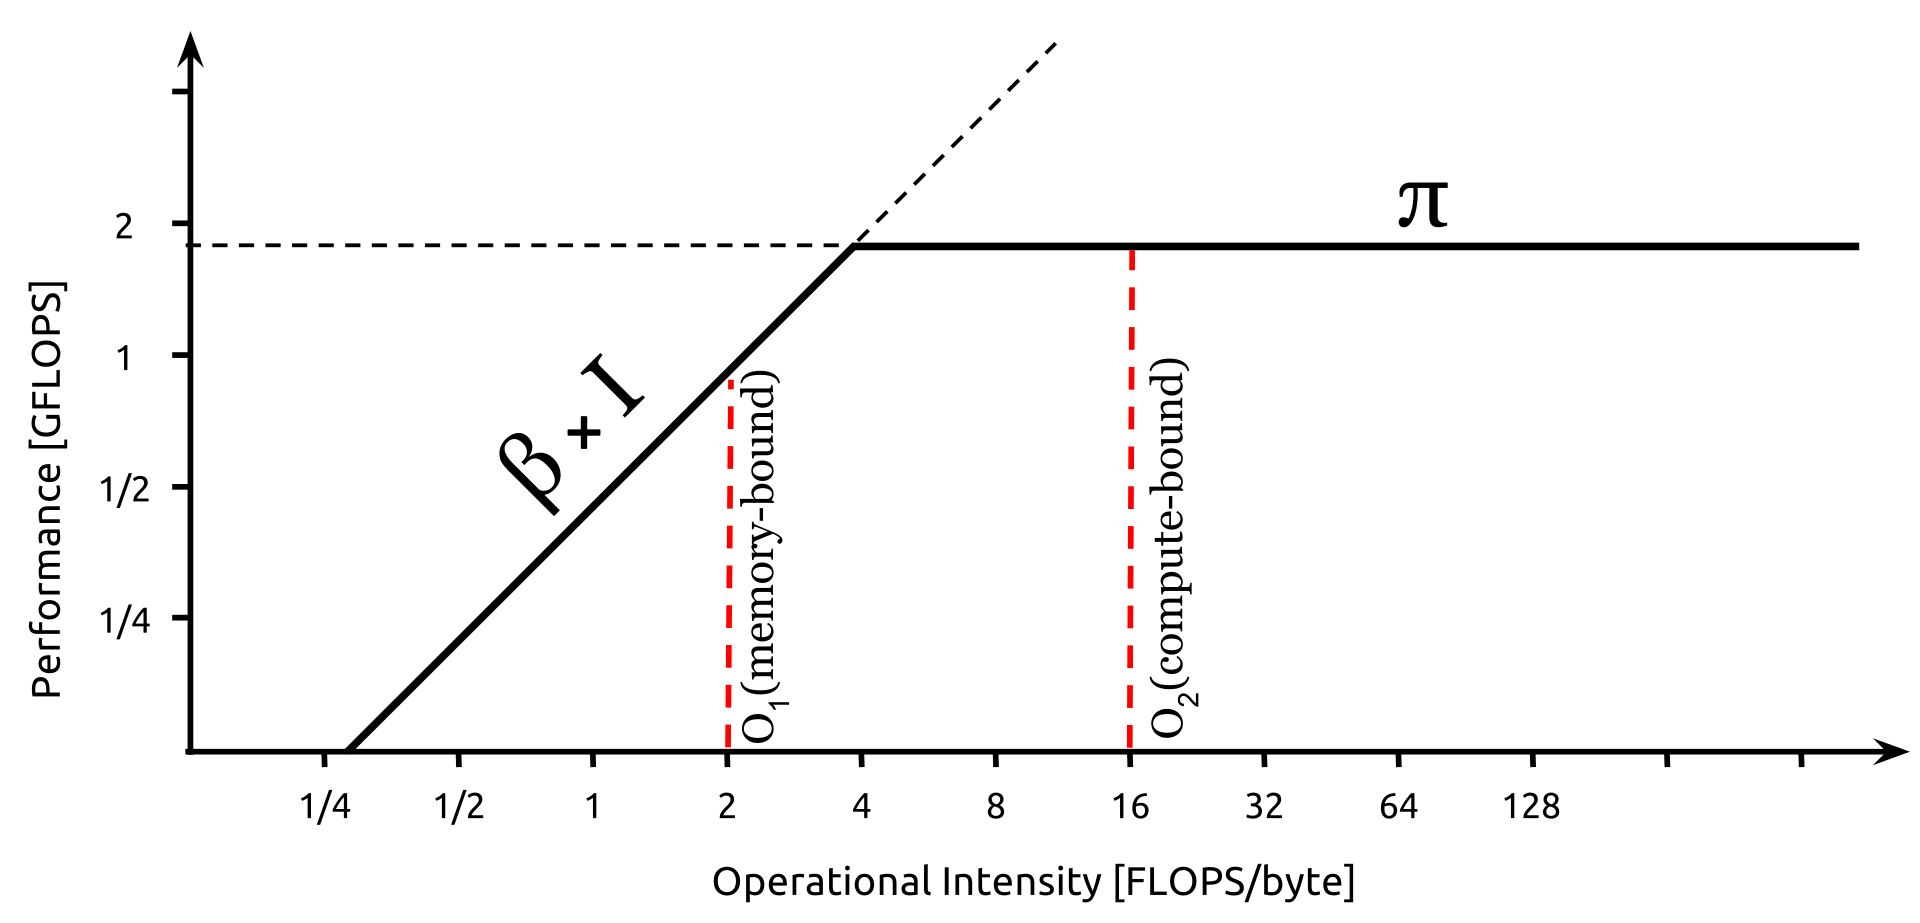
\includegraphics[height=0.4\textwidth]{chapter1/pictures/roofline_model_0.png}
    		\caption[Roofline Modell - naiv]{Die Performance $P$ als Funktion der arithmetischen Intensität $I$ bei doppelt-logarithmischer Skalierung. (naives Modell) \autocite{wikiRLM}}
    		\label{1:rl0}
		\end{figure}

		\begin{figure}[t]
		\centering
	    	
\includegraphics[height=0.4\textheight]{chapter1/pictures/roofline_model_1.png}
    		\caption[Roofline Modell - \textit{bandwidth ceiling}]{Die Performance $P$ als Funktion der arithmetischen Intensität $I$ bei doppelt-logarithmischer Skalierung. Es existiert ein negativer Offset aufgrund von \textit{bandwidth ceiling}. Dieses Verhalten entsteht durch fehlende Speicheroptimierung. \autocite{wikiRLM}}
    		\label{1:rl1}
		\end{figure}
	
		\begin{figure}[t]
		\centering
	    	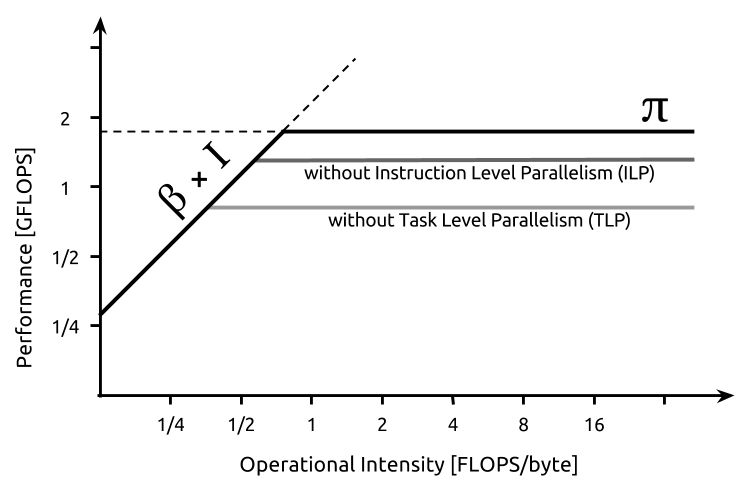
\includegraphics[height=0.35\textheight]{chapter1/pictures/roofline_model_2.png}
    		\caption[Roofline Modell - \textit{in-core ceiling}]{Die Performance $P$ als Funktion der arithmetischen Intensität $I$ bei doppelt-logarithmischer Skalierung. Es existiert ein e Beschränkung der \textit{peak performance} aufgrund von \textit{in-core ceiling}. \autocite{wikiRLM}}
    		\label{1:rl2}
		\end{figure}

		\begin{figure}[b]
		\centering
    		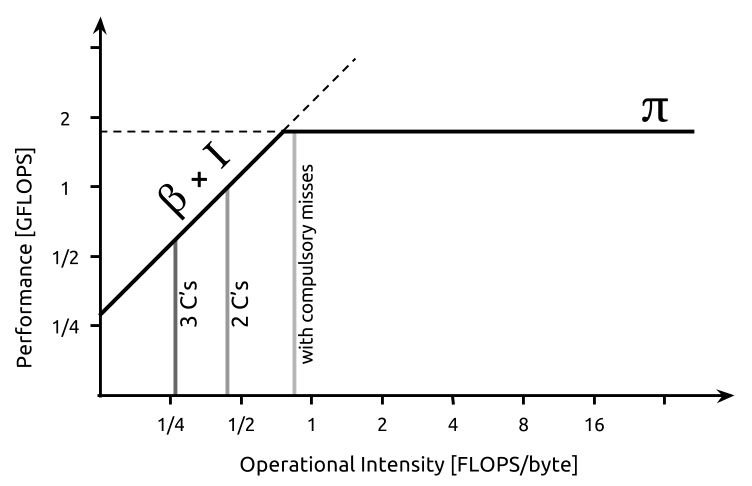
\includegraphics[height=0.35\textheight]{chapter1/pictures/roofline_model_3.png}
	    	\caption[Roofline Modell - \textit{locality walls}]{Die Performance $P$ als Funktion der arithmetischen Intensität $I$ bei doppelt-logarithmischer Skalierung. $I$ lässt sich aufgrund der Cachetopologie über bestimmte \textit{locality walls} hinaus nicht steigern. rechts: \textit{compulsory misses}, C3: zusätzlich \textit{capacity-} und \textit{conflict misses}, C2: zwei von drei \autocite{wikiRLM}}
    		\label{1:rl3}
		\end{figure}
		
		Sei eine \Gls{Arbeit} $W$ gegeben, die ein Programm oder auch nur eine bestimmte Funktion verrichten muss. $W$ wird üblicherweise angegeben in einer Zahl an Fließpunktoperationen (engl. floating point operations, FLOPs). Abhängig von der Problemstellung kann aber auch ein anderes Maß gewählt werden. $W$ ist eine Eigenschaft des Programms und hängt daher nur unwesentlich von der Hardware ab.
		
		Der \Gls{Datenverkehr} $Q$ (engl. memory traffic) bezeichnet die Zahl an Bytes, die während des Ausführens des Programms insgesamt transferriert wird. $Q$ ist im Wesentlichen eine Eigenschaft der Hardware und hängt z.B. von der Cachehierarchie ab.

		$I = W/Q$ bezeichnet die \gls{arithmetische Intensität}. Dabei handelt es sich um die Anzahl an Operationen pro transferriertes Byte. Die Einheit ist FLOPs/Byte.
		Das sogenannte naive Roofline Modell geht von nur zwei Parametern aus, der \textit{\Gls{Peak Bandwidth}} $\beta$ und der \textit{\Gls{Peak Performance}} $\pi$. Lediglich $I$ ist variabel. Die \textit{\Gls{Peak Performance}} ist eine feste Hardwaregröße, die vom ausführenden Gerät abhängt. Diese Größe lässt sich aus den entsprechenden Datenblättern ablesen. Die \textit{\Gls{Peak Bandwidth}} wird normalerweise durch \textit{benchmarking} bestimmt (später mehr). Die erreichbare \Gls{Performance} kann dann wie folgt berechnet werden:
		\begin{equation}
			P = \min \left\{ \begin{array}{ll} \pi \\
			\beta\times I \\ \end{array}\right.
		\end{equation}
		
		Abbildung \ref{1:rl0} zeigt dieses Verhalten exemplarisch. Der Schnittpunkt der beiden Linien $I^{\prime} = \pi/\beta$ wird als \textit{ridge point} bezeichnet und charakterisiert die eingesetzte Hardware entscheidend. Er bezeichnet jenes $I$, das ein Programm mindestens erreichen muss, um bei gegebener Hardware diese maximal auszureizen. Gleichzeitig beschreibt er den Punkt, ab der eine Erhöhung von $I$ keinen Effekt mehr hat. Bei Programmen, für die $I < I^{\prime}$ gilt, spricht man von \textit{memory bound}, andernfalls von \textit{compute bound}.
		
		Beim naiven Modell handelte es sich um eine best-case Abschätzung. In der Praxis gibt es allerdings weitere Limitierungen. Die Abbildungen \ref{1:rl1}, \ref{1:rl2} und \ref{1:rl3} zeigen folgende Fälle:
		
		\begin{enumerate}		
			\item Kommunikation: bandwidth ceilings
			\item Berechnung: in-core ceilings
			\item Lokalität: locality walls
		\end{enumerate}			
    \stopcontents[Einführung in High-Performance-Computing]
    
    \startcontents[Hardwaregrundlagen]
    \printcontents[Hardwaregrundlagen]{l}{1}{\chapter*{Hardwaregrundlagen}\setcounter{tocdepth}{2}}
    	\chapter{Hardwaregrundlagen}
		\section{Flynn's Taxonomy}
		Aus Wikipedia \autocite{wikiFT}:
		
		Die Flynn’sche Taxonomie wurde 1966 von Michael J. Flynn publiziert und beschreibt eine grobe Unterteilung von Rechnerarchitekturen basierend auf der Anzahl der Befehls- (instruction streams) und Datenströme (data streams). Die Klassifikation teilt im Wesentlichen vier Bereiche ein:
		
		\begin{itemize}
		\item \textbf{Single Instruction, Single Data (SISD)}\\ Unter SISD-Rechnern versteht man traditionelle Einkernprozessor-Rechner, die ihre Aufgaben sequentiell abarbeiten. SISD-Rechner sind z. B. Personal-Computer (PCs) oder Workstations, welche nach der Von-Neumann- oder der Harvard-Architektur aufgebaut sind. Bei ersterer wird für Befehle und Daten die gleiche Speicheranbindung verwendet, bei letzterer sind sie getrennt. 
		
		\item \textbf{Single Instruction, Multiple Data (SIMD)}\\ Eine Architektur von Großrechnern beziehungsweise Supercomputern. SIMD-Computer, auch bekannt als Array-Prozessoren oder Vektorprozessor, dienen der schnellen Ausführung gleichartiger Rechenoperationen auf mehrere gleichzeitig eintreffende oder zur Verfügung stehende Eingangsdatenströme und werden vorwiegend in der Verarbeitung von Bild-, Ton- und Videodaten eingesetzt.

Dies ist sinnvoll, weil in diesen Bereichen die zu verarbeitenden Daten meist hochgradig parallelisierbar sind. So sind z. B. bei einem Videoschnitt die Operationen für die vielen einzelnen Bildpunkte identisch. Theoretisch optimal wäre hier die Ausführung durch einen einzigen, auf alle Punkte anzuwendenden Befehl.

Des Weiteren sind im Multimedia- und Kommunikationsbereich erforderliche Operationen häufig keine einfachen, einzelnen Operationen, sondern eher umfangreichere Befehlsketten. Das Einblenden eines Bildes vor einem Hintergrund ist beispielsweise ein komplexer Vorgang aus Maskenbildung mittels XOR, Vorbereitung des Hintergrundes mittels AND und NOT, sowie der Überlagerung der Teilbilder durch OR. Dieser Anforderung wird durch die Bereitstellung neuer komplexer Befehle entsprochen. So vereinigt z. B. der MMX-Befehl PANDN eine Invertierung und Und-Verknüpfung der Form x = y AND (NOT x).

Viele moderne Prozessorarchitekturen (wie PowerPC und x86) beinhalten inzwischen SIMD-Erweiterungen, das heißt spezielle zusätzliche Befehlssätze, die mit einem Befehlsaufruf gleichzeitig mehrere gleichartige Datensätze verarbeiten.

Allerdings muss man zwischen Befehlen unterscheiden, die lediglich gleichartige Rechenoperationen ausführen und anderen, die bis in den Bereich der DSP-Funktionalität hineinreichen (beispielsweise ist AltiVec in dieser Hinsicht wesentlich leistungsfähiger als 3DNow). 

    \item \textbf{Multiple Instruction, Single Data (MISD)}\\ Eine Architektur von Großrechnern bzw. Supercomputern. Die Zuordnung von Systemen zu dieser Klasse ist schwierig, sie ist deshalb umstritten. Viele sind der Meinung, dass es solche Systeme eigentlich nicht geben dürfte. Man kann aber fehlertolerante Systeme, die redundante Berechnungen ausführen, in diese Klasse einordnen. Ein Beispiel für dieses Prozessorsystem ist ein Schachcomputer.

Eine Umsetzung ist das Makropipelining, bei dem mehrere Recheneinheiten hintereinander geschaltet sind. Eine weitere sind redundante Datenströme zur Fehlererkennung bzw. -korrektur. 

    \item \textbf{Multiple Instruction, Multiple Data (MIMD)}\\ Eine Architektur von Großrechnern bzw. Supercomputern. MIMD-Computer führen gleichzeitig verschiedene Operationen auf verschieden gearteten Eingangsdatenströmen durch, wobei die Verteilung der Aufgaben an die zur Verfügung stehenden Ressourcen, meistens durch einen oder mehrere Prozessoren des Prozessorverbandes, selbst zur Laufzeit durchgeführt wird. Jeder Prozessor hat Zugriff auf die Daten anderer Prozessoren.

Man unterscheidet eng gekoppelte Systeme und lose gekoppelte Systeme. Eng gekoppelte Systeme sind Mehrprozessorsysteme, während lose gekoppelte Systeme Multicomputersysteme sind.

Multiprozessorsysteme teilen sich den vorhandenen Speicher und sind somit also ein Shared-Memory-System. Diese Shared-Memory-Systeme lassen sich weiter in UMA (uniform memory access), NUMA (non-uniform memory access) und COMA (cache-only memory access) unterteilen.

Man versucht bei MIMD eine Problemstellung durch die Lösung von Teilproblemen in den Griff zu bekommen. Dabei entsteht wiederum das Problem, dass verschiedene Teilstränge des Problems miteinander synchronisiert werden müssen.

Ein Beispiel in diesem Falle wäre das UNIX-Kommando make. Hier können auch mit mehreren Prozessoren mehrere zusammengehörige Programmcodes gleichzeitig in Maschinensprache übersetzt werden. 
        \end{itemize}
        
        \section{Aufbau einer Grafikkarte}
        Auch wenn das Moor'sche Gesetz noch ansatzweise erfüllt ist, stagniert die Leistung von einzelnen Prozessoren seit Jahren (Abb. \ref{2:hard}). Folglich versucht man viele Prozessoren zu einem großen Verbund zusammen zu schalten.
        
        \begin{figure}[h]
			\centering
    		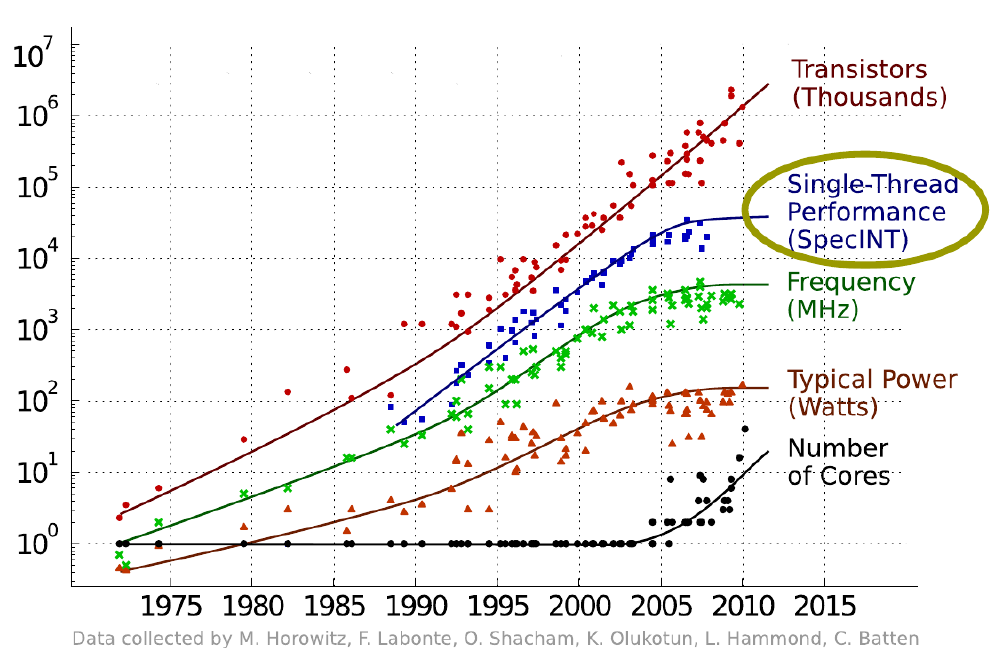
\includegraphics[height=0.6\textwidth]{chapter2/pictures/perf.png}
    		\caption[Hardware]{Entwicklung der Hardware}
    		\label{2:hard}
		\end{figure}

		Die Idee: nutze Grafikkarten als co-Prozessoren. Eine Grafikkarte besteht aus mehreren Teilen (Abb. \ref{2:graka}):
		\begin{itemize}
			\item \textbf{Bus Interface}: steuert den Datenfluss von der \Gls{PCIe}-Schnittstelle, Instruktionen werden an die GPU weitergeleitet, Speicherallozierungen an den Speichercontroller
			\item \textbf{Speichercontroller}: ein kleiner Mikroprozessor, der Speicher alloziert
			\item \textbf{Speicher}: beinhaltet den globalen und Texturspeicher. Die interne Speicherbandbreite liegt heutzutage bei bis zu 1TB/s (HBM2).
			\item \textbf{GPU}: das Herzstück der Grafikkarte. Ursprünglich war die einzige Aufgabe, der CPU 3d-Berechnungen für Texturen abzunehmen. Es existieren Grafikkarten mit zwei GPUs.
			\item \textbf{Video-Out-Controller}: wandelt die Berechnungen der GPU in Signale für die Videoausgänge um. Ein DAC Wandler wird nur für den VGA-Ausgang benötigt und existiert auf modernen Karten nicht mehr. 			
		\end{itemize}
		Auf jeder GPU sitzt ein passiv-Kühler sowie ein seperater Lüfter. Abbildung \ref{2:gpucpu} zeigt eine Grafikkarte verbaut in einem gewöhnlichen Desktop-Computer. 
		
		Datenverkehr zwischen CPU und GPU erfolgt meistens über \Gls{PCIe}x16 mit einer maximalen physikalischen Bandbreite von 32GB/s (25GB/s ohne Overhead). Sehr hochwertige Karten sind über \gls{nvlink} miteinander verbunden bei einer \Gls{Peak Bandwidth} von 300GB/s, was immer noch weit unter der internen Speicherbandbreite liegt. Kopieranweisungen zwischen CPU und GPU sollte also auf das Minimum reduziert werden.
		
		\begin{figure}[h]
			\centering
    		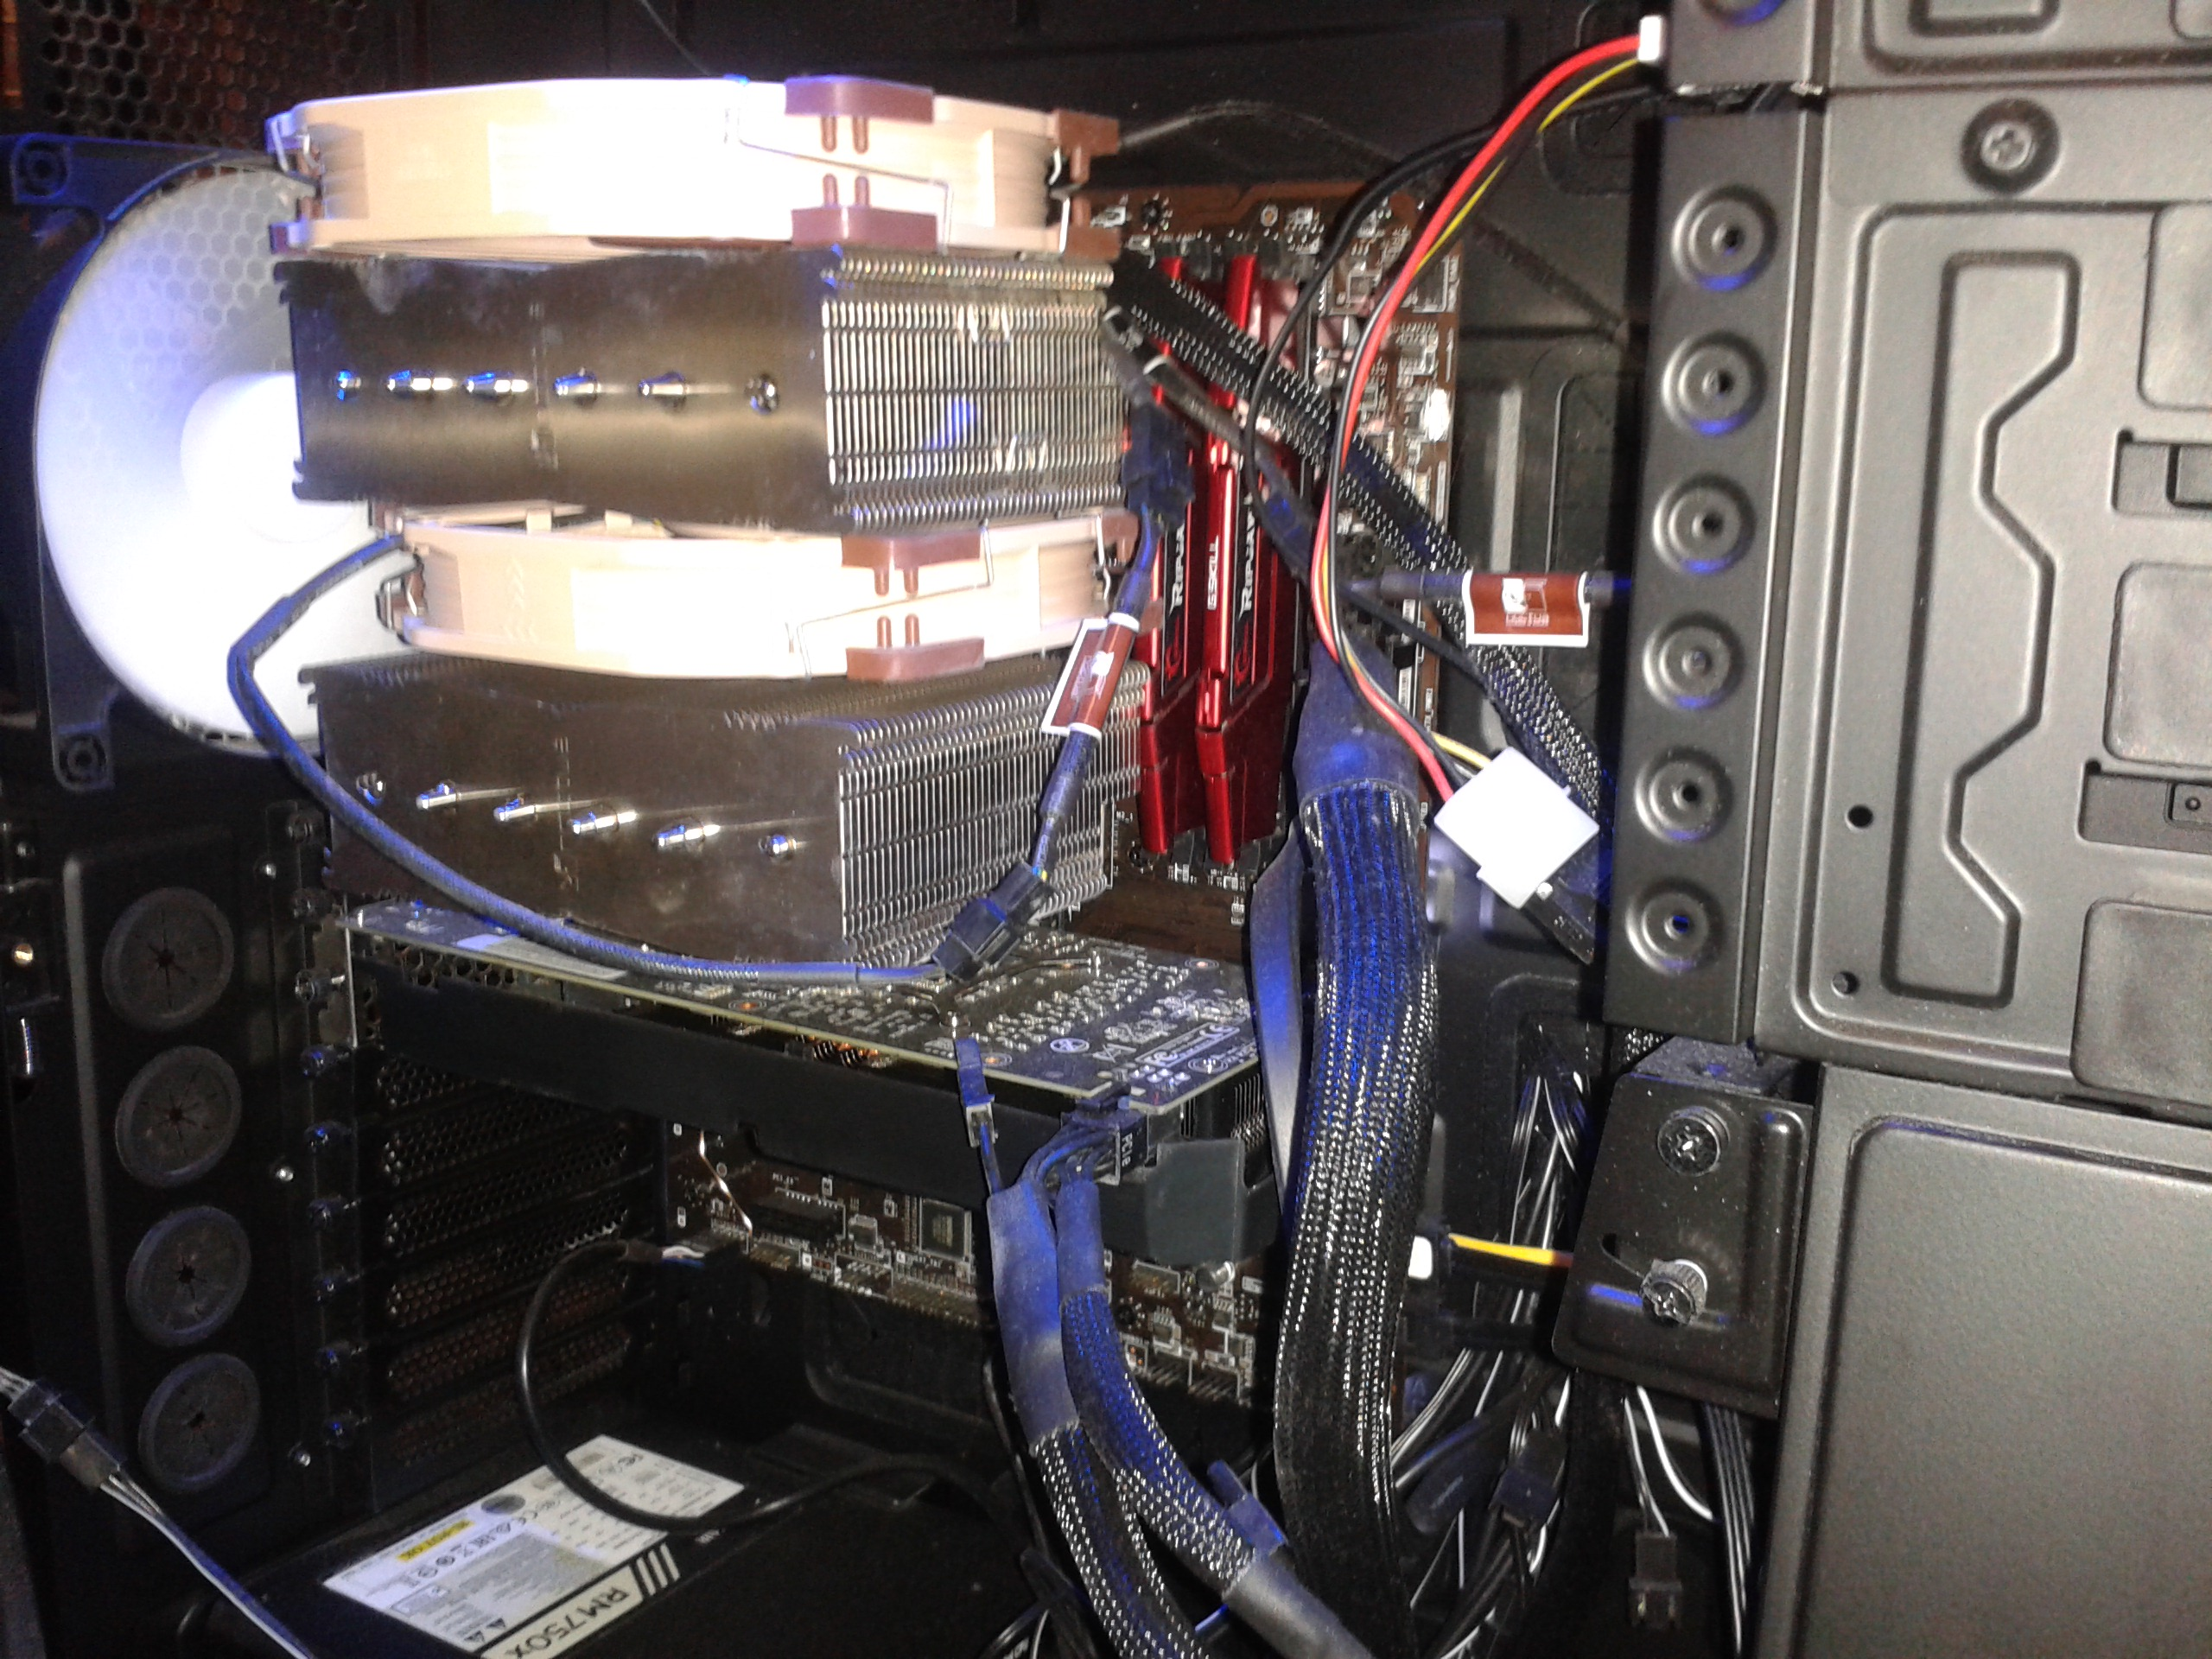
\includegraphics[height=0.6\textwidth]{chapter2/pictures/pc.jpg}
    		\caption[Desktop PC]{Aufbau eines gew\"ohnlichen Desktop-Computers}
    		\label{2:gpucpu}
		\end{figure}
		
		Nvidia bietet im Wesentlichen drei Produktlinien an:
		\begin{itemize}
		\item \textbf{GeForce}: Gaming-Grafikkarten. Berechnungen für Gaming beschränken sich meist auf das Berechnen von Texturen und Ausgabe auf dem Bildschirm. Daher sind diese Karten nicht mit einem Rechenwerk für doppelte Präzision ausgestattet und verlieren einen erheblichen Faktor bei der Performance ($\approx 32$), sollte man 64Bit Arithmetik anwenden.
		
		\item \textbf{Quadro}: Ausgestattet für HPC. Diese verlieren nur den Faktor zwei bei doppelter Präzision. Verwendet werden diese für CAD (Differentialgleichungen lösen und grafisch anzeigen für Belastungsanalysen) oder grafische Simulationen.
		
		\item \textbf{Tesla} wie Quadro, aber ohne Video-Controller. Diese sind im Wesentlichen für Deep-Learning Techniken gedacht. Moderne GPUs beinhalten sogenannte Tensorkerne, die für deep-convolutional neural networks optimiert sind. Diese kommen nun vermehrt in Gaming-Karten als Unterstützung für Ray-Tracing Kerne zum Einsatz.
		\end{itemize}		 		
		
        Karten aller drei Linien werden nach ihrer Chiparchitektur klassifiziert. Von der ältesten zur modernsten heißen diese: Tesla (nicht verwechseln!), Fermi, Maxwell, Kepler, Pascal, Volta (Weiterentwicklung: Turing)
        
        Zudem existieren Unterkategorien, die in der sogenannten \textit{\gls{compute capability}} zum Ausdruck kommen. Diese ist die wesentlichste Kenngröße einer Nvidia Grafikkarte, da sie bestimmt, welche Features von CUDA in Hardware auf der GPU implementiert sind.		
		
        \begin{figure}[h]
			\centering
    		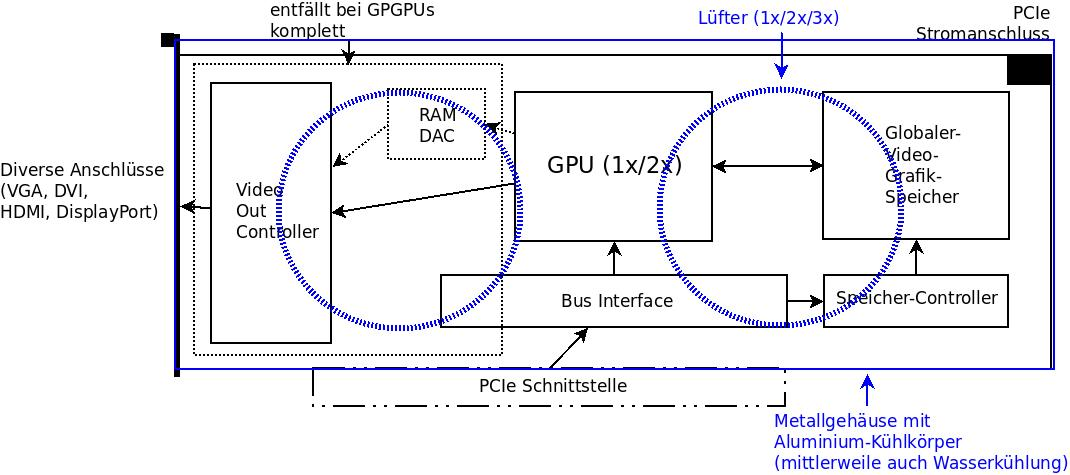
\includegraphics[width=\textwidth]{chapter2/pictures/gpu.jpg}
    		\caption[Grafikkarte]{Teile einer Grafikkarte}
    		\label{2:graka}
		\end{figure}
		
		Eine GPU ist im Wesentlichen ein Verbund aus tausenden Kernen, sogenannten \Glspl{Thread}, mit relativ geringer Leistung. Nach dem SIMD Prinzip führen alle Kerne ähliche Tätigkeiten aus. Die Idee hinter HPC auf GPUs ist, die massive Parallelität für Tätigkeiten auszunutzen, die bestimmte Eigenschaften erfüllen:
		\begin{itemize}
			\item Probleme mit extrem hoher Parallelität, z.B. sehr große unabhängige Schleifen.
			\item Probleme mit sehr vielen ähnlich gelagerten Berechnungen, also die selben Operationen in der gleichen Reihenfolge aber mit unterschiedlichen Daten.
			\item Probleme mit einer geringen \Gls{Arbeit} in jedem parallelen Prozess, z.B. einfache mathematische Formeln.
			\item Probleme mit geringem Speicherfluss.			
		\end{itemize}
			
		\begin{figure}[h]
			\centering
    		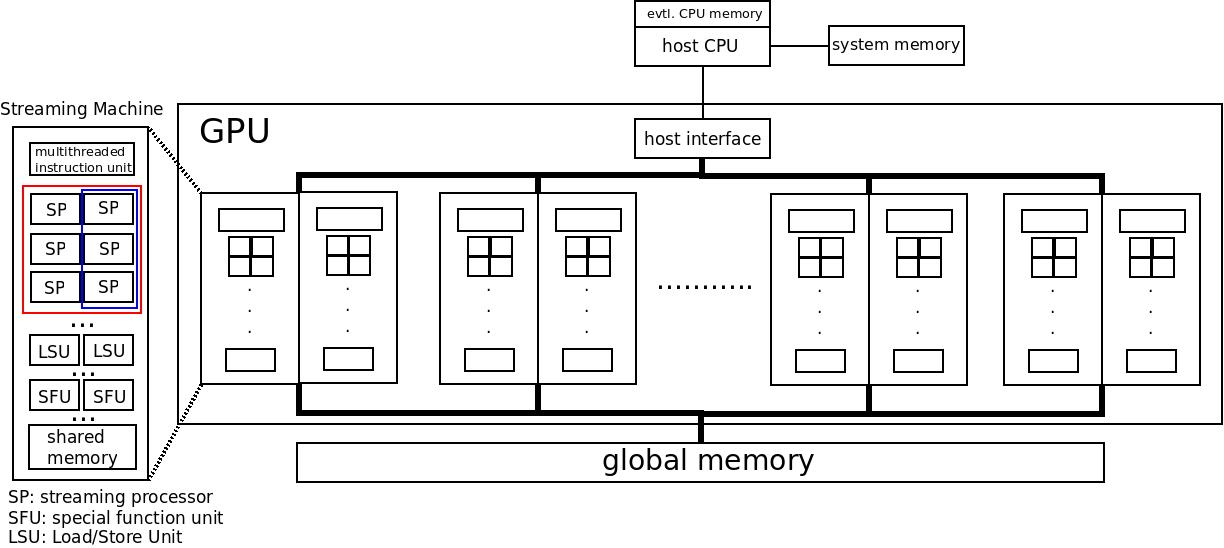
\includegraphics[width=\textwidth]{chapter2/pictures/sm.jpg}
    		\caption[GPU]{Aufbau einer GPU}
    		\label{2:gpu}
		\end{figure}
		
		Eine GPU wird aufgeteilt in eine bestimmte Anzahl von sogenannten Streaming Multiprocessors (\Gls{SM}). Üblich ist eine geringe zweistellige Anzahl (Abb. \ref{2:gpu}). Diese bestehen wiederum aus den folgenden Komponenten:
		
		\begin{itemize}
		\item Multiple Threaded Instruction Unit (\Gls{MTIU}): veteilt die Instruktionen auf einen \Gls{Thread} pro \Gls{Warp}
		\item \Glspl{Warp}: ein Verbund von 32 \Glspl{Thread}. Eine Instruktion wird kopiert und an alle weitergegeben.
		\item \Gls{Halfwarp}: Genau eine Hälfte eines \glspl{Warp}
		\item Special Function Unit (SFU): Erledigt besondere Aufgaben, z.B. shader Berechnungen (später mehr) 
		\item \Gls{shared Memory}: ein kleiner, extrem schneller Speicher, den sich alle \Glspl{Thread} eines \Gls{SM}s teilen.
		\end{itemize}

		Es ist wichtig, die technischen Details der Hardware zu kennen, um die Software darauf anzupassen. Ein HPC Programm ist üblicherweise genau auf die Hardware zugeschnitten, auf der das Programm laufen soll. Die Generalisierung eines Problems ist nicht trivial und manchmal sogar unmöglich oder nur unter starken \Gls{Performance}verlusten zu erreichen.	
    \stopcontents[Hardwaregrundlagen]
	
    \startcontents[Einführung in Nvidia CUDA]
    \printcontents[Einführung in Nvidia CUDA]{l}{1}{\chapter*{Einführung in Nvidia CUDA}\setcounter{tocdepth}{2}}
    	\chapter{Einf\"uhrung in Nvidia CUDA}
	Seit 2007 existiert das Nvidia Produkt \textit{Compute Unified Device Architecture} (CUDA). Dabei handelt es sich um eine Programmiersprache, eine Compilerarchitektur, eine Runtime-Library oder kurz um eine Platform. CUDA lässt sich mit dem Nvidia CUDA Toolkit leicht auf Linux, MacOS oder Windows installieren und bringt dabei mehrere HPC Bibliotheken mit. Auf einige soll später noch eingegangen werden. Die wichtigsten Vertreter sind:
	\begin{itemize}
		\item \textbf{cuBLAS}:   Die CUDA Implementierung der \textit{Basic Linear Algebra Subprograms}.
		\item \textbf{curand}:   Ein Zufallszahlen-Generator (RNG) und verschiedene Verteilungen.
		\item \textbf{cuSOLVER}: Eine Implementierung der beliebtesten Matrixzerlegungen.
		\item \textbf{THRUST}:   Die CUDA Implementierung der C++ Standard Template Library (STL).
	\end{itemize}
	Andere prominente Vertreter sind cuDNN, TensorRT und offizielle Partnerprojekte wie MAGMA, GROMACS oder Tensorflow.
				
		
		\section{C Runtime}
		Ein Hauptprogramm auf der CPU wird üblicherweise in C oder C++ geschrieben. Wahlweise lässt sich auch ein \Gls{API} in einer anderen Programmiersprache benutzen, z.B. pyCUDA in Python. Dieses Programm läuft wie gewohnt auf der CPU und wird fortan als Hostcode bezeichnet. Eine sehr rechenintensive Stelle im  Hostcode soll nun auf die GPU ausgelagert werden. Im gleichen Quellcode wird nun in der Programmiersprache CUDA ein sogenanntes \Gls{Kernel} definiert.
			\subsection*{Kernels}
			\Glspl{Kernel} sind sehr kleine Recheneinheiten, die parallel auf der GPU ausgeführt werden sollen. Der folgende Code zeigt ein \Gls{Kernel} zur Addition zweier Vektoren.
	  		\begin{lstlisting}[caption=~Vektoraddition Kernel]
				__global__ void VecAdd(float* A, float* B, float* C, int N)
				{
    				int i = threadIdx.x;
    				if (i < N)
        				C[i] = A[i] + B[i];
				}
				
				...
				
				int main()
				{		
					...
					VecAdd<<<1, N>>>(A, B, C, N) ;
					...
				}
			\end{lstlisting}
			
			\Glspl{Kernel} werden immer mit dem Keyword \li`__global__` deklariert und der return Typ ist immer \li`void`. \Gls{Kernel}aufrufe erfolgen asynchron, d.h. die CPU schickt den Auftrag lediglich ab und arbeitet dann weiter den Hostcode ab. Mehrere \Gls{Kernel}aufrufe hintereinander werden auf der GPU serialisiert.
			
			Die spitzen Klammern geben an, mit welchen \Glspl{Thread} der Code ausgeführt werden soll. Im obigen Fall wird das \Gls{Kernel} mit $N$ \Glspl{Thread} gestartet. Ausnahmslos jeder dieser \Glspl{Thread} erhält das \Gls{Kernel} und führt den Code aus: Jeder \Gls{Thread} rechnet sich seinen Index aus (entspricht dem Prozessor-rank). Jeder \Gls{Thread} nimmt einen Wert von A und B, rechnet die Summe aus und schreibt genau einen Wert von C. Ein \Gls{Kernel} kann man sich also so vorstellen, als würde man eine Schleife ausrollen und jedes Element einzeln und parallel berechnen. \Glspl{Kernel} können nicht auf Hostcode zugreifen.
			
			Zur besseren Steuerung der \Glspl{Thread} teilt man diese in \Glspl{Block} ein:
			
			\newpage 
			
			\begin{lstlisting}[caption=~Kernelaufruf]		
				int main()
				{
					int threadsPerBlock = 32;
					int blocksPerGrid = N / threadsPerBlock;
					
					...
					
					VecAdd<<<blocksPerGrid, threadsPerBlock>>>(A, B, C, N);
					
					...					
				}
			\end{lstlisting}

			In diesem Beispiel übergibt man im ersten Element zwischen den spitzen Klammern die Zahl an \Glspl{Block}n und im zweiten die Zahl an \Glspl{Thread} pro \Gls{Block}. Beide Zahlen multipliziert ergeben also die Zahl an \Glspl{Thread} insgesamt. Mittels \li`blockIdx.x*blockDim.x + threadIdx.x` berechnet man den globalen Index eines \Glspl{Thread}. Die \Glspl{MTIU} verteilen die \Glspl{Block} dann automatisch auf die \Gls{SM}. Sollten mehr \Glspl{Thread} involviert werden als tatsächlich zur Verfügung stehen, so wird zuerst eine passende Anzahl verteilt und dann für die restlichen \Glspl{Block} wiederholt. Der Index zählt dabei korrekt weiter, da er von der ID des \Gls{Block}s abhängt.
			
			Falls das \Gls{Kernel} eine Funktion aufrufen soll, so muss diese extra für das Device geschrieben werden. Dazu deklariert man diese Funktionen mit dem Keyword \li`__device__`. Analog dazu werden gewöhnliche Funktionen auf der CPU mit \li`__host__` deklariert. Wird kein Keyword geschrieben, so handelt es sich um eine Host Funktion. Wird eine Funktion mit beidem deklariert, so wird die Funktion für Device und Host kompiliert. Device Funktionen können nicht vom Host gerufen werden und umgekehrt. Eine Device Funktion darf einen return Wert haben.
			
			\subsection*{C++ Kompatibilit\"at}
			Die Programmiersprache CUDA orientiert sich an C11. Es können alle Features dieses Standards benutzt werden. C++ Code als Device Code zu schreiben ist allerdings wesentlich schwieriger und wurde daher nur teilweise implementiert. Eine Liste der C++ Features enthält der CUDA Programming Guide in Anhang F. \autocite{cudaPG} 
			
			
		\section{Speichermodell}
		Eine GPU kennt mindestens fünf Arten von Speicher:
		\begin{itemize}
			\item \Gls{global Memory}: Daten, die vom CPU Speicher kopiert werden, werden in diesem gespeichert. Dieser Speicher ist ausnahmslos allen \Glspl{Thread} zugänglich.
			\item \Gls{constant Memory}: Ein ebenfalls globaler Speicher. Konstante Variablen werden so read-only abgespeichert und verhalten sich ähnlich den konstanten Variablen in C (Vermeidung von Bankkonflikten).
			\item \Gls{local Memory}: Jeder \Gls{Thread} verfügt über einen sehr kleinen Speicher für Hilfsvariablen, die nur diesem zugänglich sind. Definiert man eine Variable im Devicecode, so wandert sie in den lokalen Speicher (z.B. der Index \li`int i`). Dieser Speicher ist ähnlich langsam wie \gls{global Memory}, wird aber in einen Cache geladen.
			\item \Gls{shared Memory}: Ein kleiner, extrem schneller Speicher, den sich jeweils die \Glspl{Thread} einer \Gls{SM} teilen. Pro \Gls{SM} ist ein Element in der GPU integriert.
			\item \Gls{texture Memory}: Ein interpolierender, globaler Speicher, der für Texturen, also multidimensionale Speicherstrukturen optimiert wurde.
		\end{itemize}
		
		Um die Vektoraddition von oben durchzuführen, muss die CPU zunächst die Vektoren in den \Gls{global Memory} kopieren. Folgendes Beispiel illustriert dies:		
		\begin{lstlisting}[caption=~Vektoraddition Host]
			uint N = 256;
			uint size = N∗sizeof(float);
			float ∗h_A = (float ∗)malloc(size);
			float ∗h_B = (float ∗)malloc(size);
			float ∗h_B = (float ∗)malloc(size);

			float ∗d_A;
			cudaMalloc(&d_A, size);
			float ∗d_B;
			cudaMalloc(&d_B, size);
			float ∗d_C;
			cudaMalloc(&d_C, size);
			
			
			cudaMemcpy(d_A, h_A, size, cudaMemcpyHostToDevice);
			cudaMemcpy(d_B, h_B, size, cudaMemcpyHostToDevice);

			int threadsPerBlock = 32;
			int blocksPerGrid = N / threadsPerBlock ;
			VecAdd<<<blocksPerGrid, threadsPerBlock>>>(d_A, d_B, d_C, N);
			cudaMemcpy(h_C, d_C, size, cudaMemcpyDeviceToHost);
			
			cudaFree(d_A); cudaFree(d_B); cudaFree(d_C);
			free(h_A); free(h_B); free(h_C);
		\end{lstlisting}	
		
		Der Befehl \li`cudaMalloc` erstellt einen Buffer der richtigen Größe im \Gls{global Memory}.
		Der Befehl \li`CudaMemcpy` kopiert dann den gesamten speicher des Hostvektors in den Devicevektor auf der Grafikkarte. Für eine einzelne Variable ($N$) ist dies nicht notwendig.
		Nachdem das Kernel abgeschickt wurde, wird der Ergebnisvektor auf den Host zurückkopiert.
		Hinter \li`cudaMemcpy` verbirgt sich ein impliziter \Gls{Kernel}aufruf, der synchron abläuft, d.h. die CPU muss warten bis das \Gls{Kernel} ausgeführt wurde. Es ist zu beachten, dass \Gls{Kernel}aufrufe normalerweise asynchron laufen, also die CPU nicht blockieren (non-blocking).	 Speicher auf dem Device wird mit \li`cudaFree` freigegeben.
		
		\Gls{shared Memory} wird mit dem Keyword \li`__shared__` deklariert. Der erste \Gls{Thread}, der in einem \Gls{Kernel} auf eine solche Instruktion trifft, legt eine Variable im \gls{shared Memory} der entsprechenden Größe an. Diese Variable teilen sich dann alle \Glspl{Thread} eines \Gls{Block}s. Existieren insgesamt $n$ \Glspl{Block}, so existieren auch $n$ verschiedene Variablen.
		\begin{lstlisting}[caption=~shared Memory statisch]
			__global__ void test()
			{
  				__shared__ int s[64];
  				...
			}
  		\end{lstlisting}

		Im Gegensatz zur statischen Variante lässt sich \gls{shared Memory} auch dynamisch allozieren:  		
  		\begin{lstlisting}[caption=~shared Memory dynamisch]
			__global__ void test()
			{
  				extern __shared__ int s[];
  				...
			}
			
			int main()
			{
				...
				int shared_memory_size = ...
				test<<<1, num_threads, shared_memory_size>>>();
				...
			}			
  		\end{lstlisting}
  		
        Dem \Gls{Kernel} muss die Größe des \gls{shared Memory} mitgegeben werden. 
        
        Sollen mehrere Arrays im \gls{shared Memory} abgelegt werden, so definiert man sich lediglich Pointer auf ein großes Gesamtarray. Der Beginn des jeweils neuen Arrays muss dabei dem Ende des vorangegangenen entsprechen.  	  		
  		\begin{lstlisting}	[caption=~shared Memory verteilt]	
			extern __shared__ int s[];
			int *integerData = s;                        
			float *floatData = (float*)&integerData[nI];
			char *charData = (char*)&floatData[nF];
			
			...
			
			test<<<gridSize, blockSize, 
				nI*sizeof(int) + nF*sizeof(float) + nC*sizeof(char)>>>(...);
		\end{lstlisting}

		Im folgenden Beispiel wird die Vektoraddition umgeschrieben, um sich die Vektoren A und B in den \gls{shared Memory} zu laden:	
		
		\newpage
		
		\begin{lstlisting}[caption=~Vektoraddition shared Memory]
			__global__ void VecAdd(float* A, float* B, float* C, int N)
			{
    			int i = blockDim.x * blockIdx.x + threadIdx.x;
    			int tid = threadIdx.x;
    			
    			__shared__ float As[blockDim.x];
    			__shared__ float Bs[blockDim.x];
    			
    			if (i < N)
    			{
    			    As[tid] = A[i];
    			    Bs[tid] = B[i];
    			    
    			    ...
    			    
        			C[i] = As[tid] + B[tid];
        		}
			}
		\end{lstlisting}
		
		Da ohnehin einmal \li`A[i]` und \li`B[i]` aus dem Speicher geladen werden müssen, ist es hier unsinnig, den Speicher überflüssigerweise zu kopieren. Allerdings könnten ja vor der Addition \li`As` und \li`Bs` noch mehrmals gebraucht werden. Die Aufgabe des Programmierers ist es nun herauszufinden, bei welcher Datengröße abhängig vom Algorithmus der \Gls{Performance}gewinn durch die höhere Bandbreite den Verlust durch das Kopieren übersteigt.
		
		\Gls{constant Memory} wird mit dem Keyword \li`__constant__` als globale Variable deklariert. Mit dem Befehl \li`cudaMemcpyToSymbol` wird diese dann in den Speicher der GPU kopiert und steht dort dann auch global zur Verfügung, muss also beim \Gls{Kernel}aufruf nicht explizit angegeben werden:
		\begin{lstlisting}[caption=~Vektoraddition constant Memory]
			__constant__ float d_A[12800];
			__global__ void VecAdd(float* B, float* C, int N)
			{
    			int i = blockDim.x * blockIdx.x + threadIdx.x;
    			if (i < N)
        			C[i] = d_A[i] + B[i];
			}
			
			...
			
			cudaMemcpyToSymbol(d_A, h_A, size);
			VecAdd<<<blocksPerGrid, threadsPerBlock>>>(d_B, d_C, N);
		\end{lstlisting}
		
		Der \gls{constant Memory} ist ebenfalls ein globaler Speicher und steht jedem \Gls{Thread} zur Verfügung. Allerdings müssen Aufrufe der selben Stelle im Speicher innerhalb eines \Glspl{Warp} nicht serialisiert werden (Bankkonflikt). Daher eignet sich dieser Speicher besonders für konstante Skalare, z.B. Naturkonstanten.
		
		\section{Mehrdimensionale Bl\"ocke}
		Bisher wurden \Gls{Kernel} immer nur mit eindimensionalen \Glspl{Block}n und \Glspl{Grid} ausgeführt. Allerdings verbirgt sich dahinter ein impliziter Typecast. Zum Beispiel wird \li`<<<1,N>>>` zu \li`<<<dim3(1,1,1), dim3(N,1,1)>>>`. \li`dim3` bezeichnet dabei eine eingebaute Datenstruktur, die aus drei vorzeichenlosen Ganzzahlen besteht. In diesem Fall gibt sie die Anzahl der \Glspl{Block} im \Gls{Grid} bzw. der \Glspl{Thread} pro \Gls{Block} in die Raumrichtungen \li`(x,y,z)` an. Das \Gls{Grid} und die \Glspl{Block} sind also keine Ketten sondern Quader von Objekten. Die Indizes der \Glspl{Block} und \Glspl{Thread} lassen sich dann Spalten-, Zeilen- und Ebenenweise abfragen: 			
		\begin{lstlisting}[caption=~Multidimensionale Blöcke]
			__global__ test()
			{
				int row = blockIdx.y * blockDim.y + threadIdx.y;
				int col = blockIdx.x * blockDim.x + threadIdx.x;
				...
			}
    		
    		...

		    dim3 dimBlock(BLOCK_SIZE, BLOCK_SIZE);
    		dim3 dimGrid(GRID_SIZE, GRID_SIZE;
    		test<<<dimGrid, dimBlock>>>();
		\end{lstlisting}
        In diesem Fall werden also \Glspl{Block} der Größe \li`BLOCK_SIZE`$\times$\li`BLOCK_SIZE` in einem \Gls{Grid} mit \li`GRID_SIZE`$\times$\li`GRID_SIZE` \Glspl{Block}n angeordnet. Bei modernen GPUs ist die Obergrenze für die Dimension der \Glspl{Block} \li`(1024,1024,64)`.
        
        Das folgende Beispiel behandelt die Matrixmultiplikation unter Zuhilfenahme von \gls{shared Memory} und Multidimensionalen \Glspl{Block}n:       
        \begin{lstlisting}[caption=~Matrixmultiplikation]
			#define BLOCK_SIZE 16
        	
			typedef struct
			{
				uint width;
				uint height;
				float* elements;
				uint stride;
			} Matrix;

			__device__ 
			float GetElement(const Matrix A, uint row, uint col)
			{
				return A.elements[row * A.stride + col];
			}

			__device__ 
			void SetElement(Matrix A, uint row, uint col, float value)
			{
				A.elements[row * A.stride + col] = value;
			}
			
			__device__
			Matrix GetSubMatrix(Matrix A, uint row, uint col) 
			{
				Matrix Asub;
				Asub.width    = BLOCK_SIZE;
				Asub.height   = BLOCK_SIZE;
				Asub.stride   = A.stride;
				Asub.elements = &A.elements[A.stride * BLOCK_SIZE * row 
					+ BLOCK_SIZE * col];
				return Asub;
			}	
			




       
			__global__ 
			void MatMulKernelShared(const Matrix A, const Matrix B, Matrix C)
			{    
    			uint blockRow = blockIdx.y;
    			uint blockCol = blockIdx.x;

    			Matrix Csub = GetSubMatrix(C, blockRow, blockCol);
    
    			float Cvalue = 0;

    			uint row = threadIdx.y;
    			uint col = threadIdx.x;

    			for (uint m = 0; m < (A.width / BLOCK_SIZE); ++m)
    			{
					Matrix Asub = GetSubMatrix(A, blockRow, m);
					Matrix Bsub = GetSubMatrix(B, m, blockCol);

					__shared__ float As[BLOCK_SIZE][BLOCK_SIZE];
					__shared__ float Bs[BLOCK_SIZE][BLOCK_SIZE];
					As[row][col] = GetElement(Asub, row, col);
					Bs[row][col] = GetElement(Bsub, row, col);

					__syncthreads();

					for (uint e = 0; e < BLOCK_SIZE; ++e)
							Cvalue += As[row][e] * Bs[e][col];

					__syncthreads();
				}

			SetElement(Csub, row, col, Cvalue);
			}
        \end{lstlisting}
        
        Abbildung \ref{fig3:matmul} zeigt klar, dass \gls{shared Memory} die bessere Alternative zu einer naiven Implementierung ist.
        
        \begin{figure}[h]
  		\centering
  		\scalebox{1.3}{
  		\begin{tikzpicture}
    		\begin{axis}[/pgf/number format/.cd, use comma, 1000 sep={}, xlabel={dimension $n$}, ylabel={computation time / sec.}, legend pos=outer north east, legend style={cells={align=left}}]
      		\addplot [draw=UR@color@12!50!black, mark=*, only marks, mark options={scale=.5}, fill=UR@color@12!50!white]   table[x index=0, y index=1]{/home/kat10110/script/chapter3/plots/matmul.dat};
      		\addlegendentry{ohne shared memory}
      		\addplot [draw=gray!50!black, mark=*, only marks, mark options={scale=.5}, fill=gray!50!white] table[x index=0, y index=2]{/home/kat10110/script/chapter3/plots/matmul.dat};
      		\addlegendentry{mit shared memory}     
    		\end{axis}
    	\end{tikzpicture}}
  		\caption[Matrixmultiplikation shared Memory]{Laufzeitvergleich von Matrixmultiplikationen der Größ e $n\times n$ mit und ohne shared Memory. Zum Einsatz kam eine \textit{Nvidia GTX 1060}.}
  		\label{fig3:matmul}
		\end{figure}
        
        Dieser Algorithmus ist nicht ohne Weiteres anwendbar, falls sich die Matrizen nicht bequem auf gleich große \Glspl{Block} verteilen lassen.
        
        Aus den genannten Beispielen ergeben sich Merkregeln für die Wahl der \Gls{Thread}zahl pro \Gls{Block}:
        \begin{itemize}
        	\item Die Anzahl sollte ein Vielfaches von 32 sein, um unregelmäßiges Arbeiten der \Glspl{Warp} zu verhindern.
        	\item Die Anzahl sollte ein Vielfaches der Anzahl von \Glspl{Thread} pro \Gls{SM} sein, um unregelmäßiges Mapping von physischem Speicher in den selben Adressraum zu verhindern.
        	\item Die Anzahl sollte so gewählt sein, dass sich die gesamte Problemgröße, also ein oder mehrere \Glspl{Grid}, exakt auf gleich große \Glspl{Block} verteilen lässt.
        	\item Die Gesamtzahl der \Glspl{Thread} im \Gls{Grid} sollte ein Vielfaches der insgesamt in Hardware zur Verfügung stehenden \Glspl{Thread} sein, um die GPU voll auszulasten.
        \end{itemize}
        
        Da in der Praxis diese Punkte kaum alle einzuhalten sind, ist ein Blackbox-Verfahren für die GPU schwer oder gar nicht zu programmieren. Man sollte also bereits bei der Erzeugung von Messdaten in einem Experiment oder in einer Simulation auf vernünftige Problemgrößen achten, andernfalls muss man mit \Gls{Performance}einbußen rechnen.
        								
		\section{Error Handling}
		Beinahe jeder \Gls{API}-Call liefert einen speziellen CUDA-Datentyp namens \li`cudaError_t`. Folgende Funktion fragt diesen Wert ab und gibt einen Fehlerstring zurück:		
		\begin{lstlisting}[caption=~Error Handling]
			#define CUDA_ERROR_CHECK

			#define CudaCheckError()  __cudaCheckError(__FILE__, __LINE__)

			inline void __cudaCheckError(const char *file, const int line)
			{
			#ifdef CUDA_ERROR_CHECK
				cudaError err = cudaGetLastError();
				if(cudaSuccess != err)
				{
					fprintf(stderr, "cudaCheckError() failed at %s:%i : %s\n",
					file, line, cudaGetErrorString(err));
					exit(-1);
				}

    			err = cudaDeviceSynchronize();
    			if(cudaSuccess != err)
    			{
        			fprintf(stderr, "cudaCheckError() with sync failed at 
        				%s:%i : %s\n",
					file, line, cudaGetErrorString(err));
					exit(-1);
				}
			#endif

				return;
			}
		\end{lstlisting}
		
		Mittels \li`cudaGetLastError` wird der letzte Fehler untersucht. Da \Glspl{Kernel} asynchron laufen, kann es nötig sein, mittels \li`cudaDeviceSynchronize` zu synchronisieren, d.h. alle \Glspl{Kernel} müssen ausgeführt worden sein, bevor die CPU weiter Code ausführen darf. Falls dies nicht nötig ist, sollte die Zeile kommentiert werden. Um Rechenzeit zu sparen, kann durch das \li`CUDA_ERROR_CHECK` Makro diese Funktion zur Compile-Zeit entfernt werden.
		
		CUDA Librarys (z.B. cuDNN oder cuRAND) definieren oft neue Datentypen für Fehler. Diese Funktion kann also in mehreren Variationen nötig sein.


		\section{Stream Processing}
		\subsection{Events}
        Um die Laufzeit zu messen, eignen sich CUDA-Events:		
		\begin{lstlisting}[caption=~Events]
			cudaEvent_t start, stop;
			cudaEventCreate(&start);
			cudaEventCreate(&stop);

			cudaEventRecord(start, 0);
			//zu messender Code//
			cudaEventRecord(stop, 0);	
		
			cudaEventSynchronize(stop);
			float milliseconds = 0;
			cudaEventElapsedTime(&milliseconds, start, stop);
		
			cudaEventDestroy(start);
			cudaEventDestroy(stop);
		\end{lstlisting}

		Mit \li`cudaEventRecord` werden zwei Events aufgezeichnet. Die null am Ende teilt die Events dem Stream mit Nummer 0 zu (siehe \ref{streams}). Wird diese Angabe unterdrückt, so werden die Aufrufe dem default-Stream zugeordnet. Nach dem Aufruf \li`cudaEventSynchronize`, also sobald das Event \li`stop` stattgefunden hat, kann mittels \li`cudaEventElapsedTime` die vergangene Zeit zwischen \li`start` und \li`stop` in Millisekunden gemessen werden.
		
		Zudem existiert \li`cudaError_t cudaEventQuery(cudaEvent_t event)`. Diese Funktion liefert dann einen Erfolg, falls das betreffende Event stattgefunden hat.
		
		Außerdem lassen sich mittels \li`cudaError_t cudaEventCreateWithFlags(cudaEvent_t* event, unsigned int flags)` Events mit Flags definieren, die sich in der Dokumentation der CUDA Runtime \Gls{API} nachlesen lassen. \autocite{cudaRTAPI}
		
      
		\subsection{Device Auswahl}
		Mittels \li`cudaGetDeviceCount` lässt sich ermitteln, über wie viele CUDA-fähige Grafikkarten die Platine, auf der die CPU sitzt, verfügt. Für jedes Gerät einzeln können dann die Eigenschaften des Geräts abgefragt werden.
		
		Die Geräte lassen sich mit \li`cudaSetDevice` manuell umschalten. Speicher der einen GPU lässt nur dann von der anderen abrufen, wenn der Peer-to-Peer Access mit \li`cudaDeviceEnablePeerAccess` aktiviert oder der Speicher explizit zwischen den GPUs kopiert wird. Die null am Ende teilt die Events dem Stream mit Nummer 0 zu (siehe \ref{streams}). Wird diese Angabe unterdrückt, so werden die Aufrufe dem default-Stream zugeordnet.
		\begin{lstlisting}[caption=~Device Peer-to-Peer Access]
			int deviceCount;
			cudaGetDeviceCount(&deviceCount);

			cudaDeviceProp deviceProp;
			cudaGetDeviceProperties(&deviceProp, 0);
			printf("Device %d has compute capability %d.%d.\n",
    			device, deviceProp.major, deviceProp.minor);
           
			cudaSetDevice(0);
			float* p0;
			cudaMalloc(&p0, size);
			test<<<...>>>(p0);
			
			cudaSetDevice(1);
			float* p1;
			cudaMalloc(&p1, size);
			test<<<...>>>(p1);
			
			
			
			cudaDeviceEnablePeerAccess(0, 0);
			test<<<...>>>(p0);
			
			cudaMemcpyPeer(p1, 1, p0, 0, size);
		\end{lstlisting}

	
		\subsection{Streams}\label{streams}
		Eine Menge von Instruktionen, die der Reihe nach abgearbeitet werden sollen, heißt \Gls{Stream}. Jene \Glspl{Stream} lassen sich beliebig erstellen und zerstören (\li`cudaStreamCreate`, \li`cudaStreamDestroy`). In folgendem Beispiel wird dynamisch eine Zahl von \Glspl{Stream} erstellt. Dann wird ein entsprechender Teil eines Gesamtarrays kopiert und ein Kernel ausgeführt. Damit dies in Reihe geschieht, werden sowohl \Gls{API}-calls als auch auch \Gls{Kernel} einem \Gls{Stream} zugeordnet.	
		\begin{lstlisting}[caption=~Streams]
			uint stream_num = ...;
			uint size = ...;	    
			float* hostPtr;
			cudaMallocHost(&hostPtr, stream_num * size);	
			//inputDevPtr allozieren und kopieren//
			cudaStream_t stream[stream_num];
			for (int i = 0; i < stream_num; ++i)
			{
				cudaStreamCreate(&stream[i]);
    			
				cudaMemcpyAsync(inputDevPtr + i * size, hostPtr + i * size,
					size, cudaMemcpyHostToDevice, stream[i]);
    			
				MyKernel <<<100, 512, 0, stream[i]>>>
					(outputDevPtr + i * size, inputDevPtr + i * size, size);
				
				cudaMemcpyAsync(hostPtr + i * size, outputDevPtr + i * size,
					size, cudaMemcpyDeviceToHost, stream[i]);
								
				cudaStreamDestroy(stream[i]);
			}
		\end{lstlisting}

		Die Idee dahinter ist, die CPU möglichst wenig zu blockieren und möglichst viele \Gls{Kernel} gleichzeitig auszuführen. Da ein normaler Kopierbefehl automatisch synchronisiert, muss die Kopie asynchron erfolgen. Mittels \li`cudaMallocHost` wird dafür sog. \gls{page-locked Memory} alloziert. Dieser Speicher darf vom Betriebssystem nicht verschoben werden und kann daher immer unter der selben Speicheradresse gefunden werden.
		
		Wird kein \Gls{Stream} angegeben, so wird der default-\Gls{Stream} verwendet.	
		
		Um die CPU auf einen bestimmten \Gls{Stream} warten zu lassen, kann \li`cudaStreamSynchronize` verwendet werden. \li`cudaStreamQuery` liefert genau dann einen Erfolg, wenn der \Gls{Stream} erfolgreich beendet worden.	
		
		\li`cudaStreamWaitEvent` beginnt mit der Ausführung eines \Glspl{Stream} erst, sobald ein bestimmtes Event aufgezeichnet wurde. Dieses Event kann ebenfalls einem \Gls{Stream} zugeordnet werden (\li`cudaEventRecord(start, stream[i])`).
		
		So lassen sich z.B. Abfragen erstellen,
		
		\li`if((cudaStreamQuery(stream[i]) == cudaSuccess) && (cudaEventQuery(stop) == cudaSuccess))...`
		
		mit denen man in Kombination mit der Device-Auswahl ganze Bäume von \Gls{Kernel}aufrufen erstellen kann. Auf Clustern kann man sich dies zu Nutze machen, um exakt den zeitlichen Ablauf von \Glspl{Kernel}s zu steuern.
		
		\newpage
		
		\subsection{Synchronisation}
		Explizite Synchronisierungsfunktionen:
		
		\begin{lstlisting}[caption=~Explizite Synchronisierung]
			__host__ cudaError_t cudaDeviceSynchronize(void)
			__host__ cudaError_t cudaStreamSynchronize(cudaStream_t)
			__host__ cudaError_t cudaEventSynchronize(cudaEvent_t)	
			__device__ void __syncthreads()
			__device__ void __syncwarp()
		\end{lstlisting}
		Erstere bildet für die CPU eine Barriere, bis sämtliche Kernels abgearbeitet wurden.
		
		Implizite Synchronisierung:
		\begin{itemize}
        	\item page-locked Host Memory Allozierung
			\item Device Memory Allozierung
			\item Setzen von Device Memory 
			\item Kopie zwischen zwei Adressen innerhalb desselben Device Memory
			\item ein beliebiges CUDA Kommando den 0-\Gls{Stream} betreffend,
			\item ein Wechsel zwischen L1/\gls{shared Memory} Konfigurationen beschrieben in \gls{compute capability} 3.x und \gls{compute capability} 7.x
		\end{itemize}
		
		\begin{figure}[h]
  		\centering
  		\scalebox{1.5}{
  		\begin{tikzpicture}
    		\begin{axis}[xlabel={dimension $n$}, ylabel={computation time / msec.}]
      		\addplot [draw=UR@color@12, mark=*, only marks, mark options={scale=.2}, fill=UR@color@12]   table[x index=0, y index=1]{/home/kat10110/script/chapter3/plots/prec.dat} node [below]{half};
      		%
      		\addplot [draw=gray!70!white, mark=*, only marks, mark options={scale=.2}, fill=gray!70!white] table[x index=0, y index=2]{/home/kat10110/script/chapter3/plots/prec.dat} node [left]{single~~~~~};
      		%
      		\addplot [draw=UR@color@12!50!black, mark=*, only marks, mark options={scale=.2}, fill=UR@color@12!50!black] table[x index=0, y index=3]{/home/kat10110/script/chapter3/plots/prec.dat} node [left]{double~~~~};    
    		\end{axis}
    	\end{tikzpicture}}
  		\caption[Axpy mit verschiedenen Präzisionen]{Laufzeitvergleich von Axpy-Operation ($\vec{y}\rightarrow a\cdot\vec{x}+\vec{y}$) der Grö\ss e $n$ mit half, single- und double-Präzision. Zum Einsatz kam eine \textit{Nvidia GTX 1060}.}
  		\label{fig3:axpy}
		\end{figure}
		
		
		\subsection*{\textcolor{red}{Divergenz}}
		Synchronisation ist nich nur aufgrund von Abhängigkeiten in Algorithmen notwendig. Wenn innerhalb eines \Glspl{Warp} zwei \Glspl{Thread} zur selben Zeit unterschiedliche Instruktionen erhalten sollen, müssen diese Anweisungen serialisiert werden. Führen innerhalb eines jeden \Glspl{Warp} die \Glspl{Thread} paarweise unterschiedliche Instruktionen aus, so verliert man den Faktor 32 in der \Gls{Performance}. Diese sogenannte Divergenz kann nach jeder if-Anweisung auftreten und sollte so schnell wie möglich durch Synchronisierung aufgelöst werden. 
		
		
		\section{Datentypen}
		Auf GPUs existiert ein zwei-byte Datentyp mit halber Präzision. Benutzt man die in CUDA eingebauten arithmetischen Funktionen, kann man die Performance dadurch weiter verbessern.			
		\begin{lstlisting}[caption=~Half Precision]
		#include<cuda_fp16.h>
		#include "fp16_conversion.h"
		
		__global__
		void haxpy(int n, half a, const half *x, half *y)
		{
    		int start = threadIdx.x + blockDim.x * blockIdx.x;
    		int stride = blockDim.x;

			int n2 = n/2;
			half2 *x2 = (half2*)x, *y2 = (half2*)y;

			for (int i = start; i < n2; i+= stride) 
					y2[i] = __hfma2(__halves2half2(a, a), x2[i], y2[i]);

			if (start == 0 && (n%2))
					y[n-1] = __hfma(a, x[n-1], y[n-1]);
		}
		\end{lstlisting}
		
	    Die benutzten Funktionen verlangen den Datentyp \li`half2`, also eine Kombination von zwei \li`half` Werten.
	    
		Eingebaute Funktionen wären z.B. \li`__hdiv`, \li`__hadd` oder \li`__hmul`. Eine Auflistung aller Funktionen befindet sich in Kapitel 1.1 der Dokumentation der CUDA Math \Gls{API}. \autocite{cudaMath}
		
		Der Header \textit{cuda\_ fp16.h} befindet sich im üblichen include-Ordner. \textit{fp16\_ conversion.h} benötigt man jedoch aus dem github: \url{https://github.com/NVIDIA-developer-blog/code-samples/blob/master/posts/mixed-precision/fp16_conversion.h}
		
		Diese Datei enthält Konvertierungsfunktionen für \li`float` nach \li`half`.
	
		
		\section{Atomic Operations und Reduktionen}
		Eine Reduktion ist eine Operation, die die Dimensionalität eines Objekts verringert. Üblicherweise sind damit Operationen gemeint, die ein Array beliebiger Größe auf ein einfaches Skalar verringern. Beispiele dafür sind die Maximumsreduktion (also das Auffinden des größten Wertes), die Minimumsreduktion, die Summenreduktion (also die Summe aller Elemente) oder das Produkt aller Elemente. 
		
		Dies impliziert, dass viele \Glspl{Thread} gleichzeitig den selben Wert aktualisieren müssen, z.B. beim Addieren einer Zahl zu einem globalen Zähler. An dieser Stelle tritt ein sogenanntes Datarace auf: Ein \Gls{Thread} liest einen Wert aus dem Speicher, addiert und legt die Variable wieder im Speicher ab und überschreibt damit einen Wert der währenddessen von anderen \Glspl{Thread} bereits bearbeitet wurde bzw. bearbeitet wird. Um diese Zugriffe zu serialisieren, stellt CUDA sogenannte Atomic Operations zur Verfügung, also Operationen, die garantiert seriell ablaufen. Beispielsweise \li`int atomicAdd(int* address, int val)` addiert auf eine Variable bei der Speicheradresse \li`address` den Wert \li`val`. Eine Liste befindet sich im Anhang B.12 des CUDA Programming Guides. \autocite{cudaPG}
		
		Diese Form der Implementierung ist sehr langsam und eher zum Debuggen gedacht. Eine parallele Methode ist erforderlich. Im Prinzip nimmt zu Beginn jeder \Gls{Thread} zwei Werte und führt die Operation aus. Der nächste \Gls{Thread} nimmt abermals zwei Werte ohne Überlapp zum Vorherigen. Nach einem Schritt hat sich die Anzahl der zu reduzierenden Elemente halbiert. Im nächsten Schritt wird mit der halben Zahl der \Glspl{Thread} abermals halbiert, bis die Reduktion bereit steht.
		
		Im Folgenden wird eine naive Implementierung mit einfachen Mitteln optimiert.
		
		--SIEHE reduction.cu--
		
		Verschiedene HPC Librarys bieten Implementierungen der gängigsten Reduktionen an, z.B. THRUST oder MAGMA. 
		
		
		\section{NVCC}
		Der Nvidia CUDA Compiler (\gls{nvcc}) wird benutzt um sowohl Host- als auch Devicecode zu kompilieren. Es handelt sich dabei um eine Obermenge des g++. Es lässt sich bis zum C++14 Standard alles in C oder C++ kompilieren. Soll explizit CUDA Code kompiliert werden, so muss die Quelldatei die Dateiendung \li`.cu` tragen. Andernfalls wird der Code als gewöhnliches C++ kompiliert und der Compiler liefert Fehler, sobald er auf Devicecode oder auf einen Aufruf der Runtime Library stößt.
		
		Der Compiler wird wie gewohnt gestartet:
		
		\li`nvcc <name>.cu`
		
		Der Compiler kompiliert nun getrennt Hostcode wie gewohnt mittels gcc/g++ (clang unter MacOS), Devicecode aber in eine assemblerartige Sprache namens \textit{Nvidia Parallel Thread Execution} (\Gls{NVPTX}). Aus dieser kann Maschinencode erstellt werden, der für die GPU lesbar ist. Im Handbuch des nvcc \autocite{cudaNVCC} findet sich eine Liste der Compilerflags. Diese sind in den wesentlichen Punkten kompatibel zu g++ mit Ausahme einiger spezieller Modi für Devicecode.
		
		Die wichtigste Ausnahme ist: \li`-arch=compute_35 -code=compute_35`
		
		Dieses lässt den Code explizit für eine \gls{compute capability} kompilieren, in diesem Fall 3.5. Damit lassen sich Features dieser \gls{compute capability} aktivieren. Allerdings ist der code auf älteren Karten dann nicht mehr ausführbar (falls modernere Features verwendet wurden). "Arch" (Architecture) bezeichnet dabei das Chipdesign, "Code" die Software.
		
		Mit \li`-c` lassen sich wie gewohnt Objektdateien (\li`.o`) und damit statische und dynamische Librarys erstellen.
		
		Der Compiler inkludiert automatisch einige Header z.B. cuda.h oder math.h, sowohl für Host- als auch für Devicecode und linkt selbstständig mit den richtigen Bibliotheken. Für weitere Bibliotheken können selbstverständlich die Compilerflags \li`-I` und -\li`-L` sowie der Linker, z.B. für \li`-lgomp` benutzt werden.
		
		Das Verhalten des Compilers kann über verschiedene Umgebungsvariablen gesteuert werden. Eine Liste befindet sich im Anhang J des CUDA Programming Guides. \autocite{cudaPG} 

    \stopcontents[Einführung in Nvidia CUDA]
		
    \startcontents[Einführung in OpenCL]
    \printcontents[Einführung in OpenCL]{l}{1}{\chapter*{Einführung in OpenCL}\setcounter{tocdepth}{2}}
    	\chapter{Einf\"uhrung in OpenCL}
	\textit{Open Computing Language} (OpenCL) ist eine freie open-source Programmierschnittstelle für paralleles Rechnen, die Von Apple im Jahr 2009 entwickelt wurde. Heute liegt diese in Version 2.2 vor und wird von der Khronos Gruppe entwickelt, der sich mittlerweile über 200 Firmen angeschlossen haben. Das Ziel hinter dem Projekt ist es, eine low-level Programmiersprache und Schnittstelle zu schaffen, mit denen sich maximal inhomogene Parallelrechner (CPUs, GPUs, Grafikchips, FPGAs, Beschleuniger, ...) programmieren lassen und dabei Plattformunabhängigkeit gewährleisten. Ein Gerät benötigt dafür eine Hardwareimplementierung und der Hersteller muss eine OpenCL Implementierung in Software bereitstellen (z.B. AMD, Intel, ...). Im Nvidia Toolkit ist eine OpenCL Installation enthalten, in Hardware aber nur für Version 1.2 implementiert. C- und C++-\Glspl{API} sind gewöhnliche Librarys, die unter Linux über die Paketquellen installiert werden können.
	
	Die Khronos Gruppe entwickelt ebenfalls die Grafikbibliothek OpenGL und Nachfolger Vulkan, für die ähnliche Prinzipien gelten. 
	 
	    \section{Begriffe}
	    Obwohl Nvidia ebenfalls Teil der Khronos Gruppe ist, haben sich in der Fachsprache hier andere Begriffe etabliert. Tabelle \ref{tab4:begriffe} zeigt typische OpenCL Begriffe und ihre Entsprechung in CUDA.
	    	\begin{table}[h]
	    		\centering
	    		\begin{tabular}{|l|l|}
	    			\toprule 
	    			\textbf{OpenCL} & \textbf{CUDA} \\ \hline\hline
	    			Workitem & Thread \\
	    			Workgroup & Block \\ \hline
	    			Global Memory & Global Memory \\
	    			Constant Memory & Constant Memory \\
	    			Local Memory & Shared Memory \\
	    			Private Memory & Local Memory \\ \hline
	    			Platform & \textit{keine} \\
	    			Device & Device \\
	    			Context & \textit{keine} \\
	    			Command Queue & Stream \\
	    			Kernel & Kernel \\
	    			Event & Event \\ \hline
	    			Global Work Size & Grid Size \\
	    			Local Work Size & Block Size \\
	    			Work Dimension & Grid/Block Dimension \\
	    			\bottomrule
	    		\end{tabular}
	    		\caption{Typische OpenCL Begriffe und ihre Entsprechung in CUDA}
	    		\label{tab4:begriffe}
	    	\end{table}
	    	Technisch gesehen sind sich AMD und Nvidia Grafikkarten ähnlich. Allerdings nennt AMD die \Glspl{Warp} \Glspl{Wavefront} und deren Größe ist abhängig vom Chip entweder 32 oder 64. Demnach sollte bei entsprechender Größe die Local Work Size, also die Größe einer \Gls{Workgroup}, ein Vielfaches von 32 oder 64 sein. 
	    	
	    	Diese Einführung beschränkt sich auf das Programmieren von GPUs. Die dafür verwendeten Befehle sind CUDA sehr ähnlich und tragen lediglich andere Namen. Tabelle \ref{tab4:begriffe} zeigt eine Auflistung der wichtigsten.
	    	
	    	\begin{table}[h]
	    		\centering
	    		\scalebox{0.9}{%
	    		\begin{tabular}{|l|l|}\toprule
	    			\textbf{OpenCL} & \textbf{CUDA} \\ \hline\hline
					\li`__kernel`, \li`kernel` & \li`__global__` \\
					\li`__constant`, \li`constant` & \li`__constant__` \\
					\li`__global`, \li`global` & \textit{automatisch} \\
					\li`__private`, \li`private` & \textit{automatisch} \\
					\li`__local`, \li`local` & \li`__shared__` \\
\hline					
					\li`get_global_id(0)` & \li`blockIdx.x*blockdim.x + threadIdx.x` \\
					\li`get_global_id(1)` & \li`blockIdx.y*blockdim.y + threadIdx.y` \\
					\li`get_global_id(2)` & \li`blockIdx.z*blockdim.z + threadIdx.z` \\
\hline					
					\li`get_local_size(0)` & \li`blockdim.x` \\
					\li`get_local_size(1)` & \li`blockdim.y` \\
					\li`get_local_size(2)` & \li`blockdim.z` \\
\hline																				
					\li`get_global_size(0)` & \li`griddim.x` \\
					\li`get_global_size(1)` & \li`griddim.y` \\
					\li`get_global_size(2)` & \li`griddim.z` \\
					
					\li`clCreateBuffer(...)` & \li`cudaMalloc(...)` \\
					\li`clEnqueueWriteBuffer(..)` & \li`cudaMemcpy(Async)(..., cudaMemcpyHostToDevice)` \\
					\li`clEnqueueReadBuffer(..)` & \li`cudaMemcpy(Async)(..., cudaMemcpyDeviceToHost)` \\
					\li`clEnqueueNDRangeKernel(..., <Kernel>, ...)`, \li`clSetKernelArg(...)` & \li`<kernelcall><<<...>>>(...)` \\
\hline
					\li`barrier(CLK_LOCAL_MEM_FENCE)` & \li`__syncthreads()` \\
					\li`barrier(CLK_GLOBAL_MEM_FENCE)` & \li`__syncthreads()` \\
					\li`barrier(CLK_IMAGE_MEM_FENCE)`\footnote{wurde in späteren Versionen in \li`work_group_barrier(...)` umbenannt} & \textit{keine} \\ \bottomrule
	    		\end{tabular}}
	    		\caption{Typische OpenCL Befehle/Keywords und ihre Entsprechung in CUDA}
	    		\label{tab4:befehle}
	    	\end{table}
	    	
	    	Für die Nvidia Produktlinien Geforce, Quadro und Tesla existieren bei AMD die Entsprechungen Radeon, Radeon Pro und Radeon Instinct. 
	    	
		\section{Programmiermodell}
		Im Gegensatz zu CUDA fordert OpenCL eine strikte Trennung von Host- und Devicecode in verschiedenen Dateien. Das Hostprogramm wird mittels der OpenCL C-\Gls{API} programmiert (oder C++ Wrapper), bei der es sich um eine gewöhnliche C-Library handelt. Dieses Hostprogramm wird mit einem beliebigen C- oder C++-Compiler übersetzt und unterstützt damit auch die modernste Features beider Programmiersprachen.
		
		Das Deviceprogramm, also die \Gls{Kernel} liegen in einer oder mehrerer seperater Dateien vor, die als String vom Hostprogramm eingelesen werden. Dies hat den Vorteil, dass zu Compilezeit der Inhalt des Programms nicht bekannt sein muss und damit auch nicht verändert wird. Erst zur Laufzeit wird unsichtbar für den Nutzer der OpenCL Compiler gerufen und das OpenCL Programm kompiliert und ausgeführt. Bei einer Änderung eines \Glspl{Kernel} muss das Hostprogramm also nicht noch ein weiteres Mal kompiliert werden.
		
		Devicecode wird in der eigentlichen Programmiersprache OpenCL C geschrieben, die sich im Wesentlichen an C99 orientiert. Teilweise wurde auch C++ unter dem Namen OpenCL C++ implementiert (siehe \ref{OCLC++}). Es folgt eine Auflistung der wichtigsten Einschränkungen:
		\begin{itemize}
		\item keine C99-Standard Header, Ersatz ist der Vorrat von built-in-Funktionen.
		\item Kernel-Zeigerargumente müssen mit \li`__global`, \li`__constant`, oder \li`__local` qualifiziert werden.  
		\item nur \li`__constant`-Zeiger dürfen \li`__constant`-Zeigern zugewiesen werden.
		\item keine Zeiger auf Funktionen.
		\item keine Bitfelder.
		\item keine VLAs (variable length arrays).
		\item weder Makros noch Funktionen mit variabler Argumentzahl (außer \li`enqueue_kernel`).
		\item keine auto und register Speicherklassen.
		\item keine rekursiven Funktionen.
		\item \Glspl{Kernel} sind immer Prozeduren mit \li`void`-Ergebnis.
		\item keine \Gls{Kernel}-Argumente mit den Typen \li`bool`, \li`half`, \li`size_t`, \li`ptrdiff_t`, \li`intptr_t`, \li`uintptr_t`, sowie Strukturen und Unions mit einer dieser Komponenten.
		\item keine Arithmetik für \li`half`, nur Speicherformat.
		\item irreduzible Anweisungsgruppen (z.B. Sprünge in Schleifen) sind implementation-defined.
		\item \li`const`, \li`restrict` und \li`volatile` sind erlaubt, aber für Images verboten.
		\item \li`event_t` darf kein \Gls{Kernel}-Argument sein.
		\item  \li`event_t` darf nicht zusammen mit \li`__local`, \li`__constant` and \li`__global` verwendet werden.
		\end{itemize}
		
			\subsection{Platformen}
			Da mehrere Verschiedene Implementierungen von OpenCL existieren, muss zunächst eine \Gls{Platform} ausgewählt werden. Die Khronos Gruppe aktualisiert stetig die Liste aller Platformen: \url{https://www.khronos.org/conformance/adopters/conformant-products/opencl}
			\newpage
			\begin{lstlisting}[caption=~Platformabfrage]
			cl_platform_id platform_id = NULL;
			cl_uint ret_num_platforms;
			clGetPlatformIDs(1,&platform_id, &ret_num_platforms);
			\end{lstlisting}

			\li`platform_id` kann bei mehreren Platformen ein Array von IDs sein. In diesem Fall muss im ersten Argument angegeben werden, nach wie vielen Platformen gesucht werden soll.
			
			Die meisten \Gls{API} Aufrufe geben einen Fehlercode zurück, der in einer Tabelle nachgeschlagen werden kann: \url{https://streamhpc.com/blog/2013-04-28/opencl-error-codes/}
			
			Im Folgenden werden nur die OpenCL eigenen Datentypen verwendet (siehe \ref{makros}).					
			\subsection{Devices}
			Jede \Gls{Platform} stellt OpenCL für ein oder auch mehrere Geräte zur Verfügung. Im nächsten Schritt müssen also die entsprechenden Devices den gefundenen \Glspl{Platform} zugeordnet werden.		
			\begin{lstlisting}[caption=~Deviceabfrage]
			cl_device_id device_id = NULL;	
			clGetDeviceIDs(platform_id, CL_DEVICE_TYPE_DEFAULT, 1, 
				&device_id, &ret_num_devices);
			\end{lstlisting}
			Auch hier kann \li`device_id` ein Vektor sein. Für den Typ des Geräts existieren folgende Möglichkeiten:
				
			\subsection{Kontexte}
			Ein \Gls{Kontext} ist ein \Gls{Handle} für das OpenCL Programm. Dieser beinhaltet Speicherobjekte, Programme und Command Queues. Folglich müssen diese also einem neu erstellten \Gls{Kontext} zugeordnet werden. Abbildung \ref{4:class} zeigt die Zusammenhänge sämtlicher OpenCL Klassen \autocite{oclRC} basierend auf Unified Modelling Language (UML). \autocite{uml}
			\begin{lstlisting}[caption=~Kontexte]
			cl_int ret;
			cl_context context = clCreateContext(NULL, 1, &device_id, 
				NULL, NULL, &ret);	
			\end{lstlisting}
			Sollte eine Funktion über einen eigenen Rückgabewert verfügen, so ist das letzte Argument üblicherweise eine Referenz auf einen Fehlercode.
			\begin{figure}[h]
				\centering
				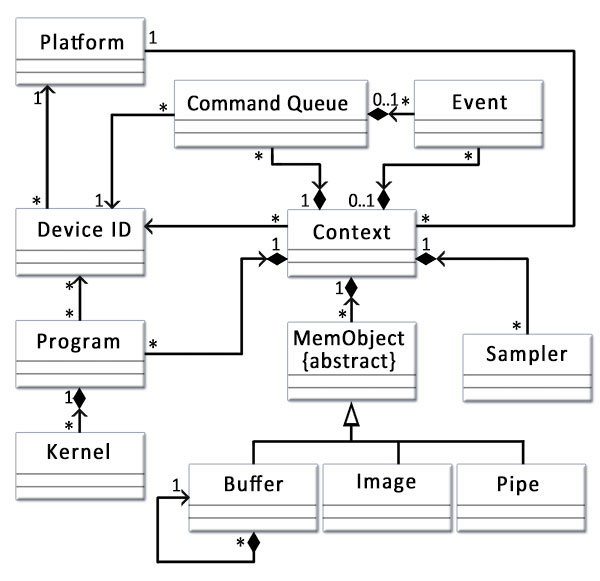
\includegraphics[width=0.7\textwidth]{/home/kat10110/script/chapter4/pictures/class.jpg}
				\caption{Zusammenhänge sämtlicher OpenCL Klassen}
				\label{4:class}
			\end{figure}				
				
			\subsection{Programme}
			Als nächstes muss das OpenCL Programm als String gelesen, zur Laufzeit kompiliert und dem Kontext hinzugefügt werden. 
			\begin{lstlisting}[caption=~OpenCL Programm]
			FILE *fp;
			char *source_str;
			size_t source_size;
			fp = fopen("cl_vecadd.cl", "r");
			if(!fp)
			{
				fprintf(stderr, "Failed to load the kernel!\n");
				exit(1);
			}
			fseek(fp, 0, SEEK_END);
			size_t s = ftell(fp);
			fseek(fp, 0, SEEK_SET); 
			source_str = (char*)malloc(s);
			source_size = fread(source_str, 1, s, fp);
			fclose(fp);
			
			cl_program program = clCreateProgramWithSource(context, 1, (const char **)&source_str, (const size_t *)&source_size, &ret);
			\end{lstlisting}
			
			Mittels \li`clBuildProgram(program, 1, &device_id, "-D name=definition -I dir", NULL, NULL)` lassen sich ähnlich dem C-Compiler dem OpenCl Compiler zusätliche Informationen mitgeben. So lässt sich der Include-Pfad erweitern. Außerdem können mit -D Makros gesetzt werden. Eine Auflistung voreingestellter Makros findet sich in Kapitel \ref{makros}.
			
			Das vorletzte Argument kann einen Pointer auf eine Funktion enthalten, die nach erfolgreichem Kompilieren ausgeführt werden soll. Das letzte Argument kann die Argumente dieser Funktion beinhalten.
			
			Da an dieser Stelle erst das eigentliche OpenCL Programm kompiliert wird, muss nun der Output des OpenCL Compilers abgefragt werden.
			
			\newpage			
			\begin{lstlisting}[caption=~Fehlerabfrage OpenCL Compiler]
			if(ret != 0){
				size_t sz; char * bf;

				clGetProgramBuildInfo(program, device_id, CL_PROGRAM_BUILD_STATUS, 
					0, NULL, &sz);
				bf = (char*)malloc((sz+1) * sizeof(char));
				if(bf)
				{
					clGetProgramBuildInfo(program, device_id, CL_PROGRAM_BUILD_STATUS, 
						sz+1, bf, NULL);
					bf[sz] = 0;
					fprintf(stderr, "\n%s\n", bf);
					free(bf);
				}

				clGetProgramBuildInfo(program, device_id, CL_PROGRAM_BUILD_OPTIONS, 
					0, NULL, &sz);
				bf = (char*)malloc((sz+1) * sizeof(char));
				if(bf)
				{
					clGetProgramBuildInfo(program, device_id, CL_PROGRAM_BUILD_OPTIONS, 
						sz+1, bf, NULL);
					bf[sz] = 0;
					fprintf(stderr, "\n%s\n", bf);
					free(bf);
				}
				
				clGetProgramBuildInfo(program, device_id, CL_PROGRAM_BUILD_LOG, 
					0, NULL, &sz);
				bf = (char*)malloc((sz+1) * sizeof(char));
				if(bf)
				{
					clGetProgramBuildInfo(program, device_id, CL_PROGRAM_BUILD_LOG, 
						sz+1, bf, NULL);
					bf[sz] = 0;
					fprintf(stderr, "\n%s\n", bf);
					free(bf);
				} }
			\end{lstlisting}
			
			\newpage
			
			\subsection{Kernel}
			Danach kann das eigentliche \Gls{Kernel} erstellt werden. Dazu muss der Name der Funktion als String übergeben werden. Das Programmieren der Kernels funktioniert ähnlich wie in CUDA.			
			\begin{lstlisting}[caption=~Kerneldefinition]
			__kernel void vecadd(__constant float *x, __constant float* y, __global float *res, const uint size)
			{
  				uint i = get_global_id(0);
  				if(i < size)
    				res[i] = x[i] + y[i];
			}
			\end{lstlisting}
			
			\Glspl{Kernel} müssen mit dem Keyword \li`__kernel` deklariert. Der Rückgabewert ist immer \li`void`. Jedes Objekt liegt per Default im \gls{private Memory} des \Glspl{Workitem}. Arrays müssen also mit dem entsprechenden Keyword deklariert werden, \li`__global` für \gls{global Memory}, \li`__constant` für \gls{constant Memory} und \li`__local` für \gls{local Memory}. Die Unterstriche können weggelassen werden. 
			
			Eine zusätlich definierte Funktion kann vom \Gls{Kernel}, also vom Device aus, wie aus C gewohnt ausgeführt werden. 
			
			Für das \Gls{Kernel} müssen wie gewohnt Buffer erstellt und Speicher kopiert werden. Zudem müssen die Kernelargumente explizit gesetzt werden.
			\begin{lstlisting}[caption=~Kernelaufruf]
			cl_mem d_x  = clCreateBuffer(context, CL_MEM_READ_ONLY, 
				size*sizeof(cl_float), NULL, &ret);
			cl_mem d_y  = clCreateBuffer(context, CL_MEM_READ_ONLY, 
				size*sizeof(cl_float), NULL, &ret);
			cl_mem d_res = clCreateBuffer(context, CL_MEM_WRITE_ONLY, 
				size*sizeof(cl_float), NULL, &ret);
			
			clEnqueueWriteBuffer(command_queue, d_x, CL_TRUE, 0, 
				size*sizeof(cl_float), h_x, 0, NULL, NULL);
			clEnqueueWriteBuffer(command_queue, d_y, CL_TRUE, 0, 
				size*sizeof(cl_float), h_y, 0, NULL, NULL);
			
			cl_kernel kernel_vecadd = clCreateKernel(program, "vecadd", &ret);
			
			
			
			clSetKernelArg(kernel_vecadd, 0, sizeof(cl_mem),  (void *)&d_x);
			clSetKernelArg(kernel_vecadd, 1, sizeof(cl_mem),  (void *)&d_y);
			clSetKernelArg(kernel_vecadd, 2, sizeof(cl_mem),  (void *)&d_res);
			clSetKernelArg(kernel_vecadd, 3, sizeof(cl_uint), &size);
			
			// Ausführen...
			\end{lstlisting}
			
			Ein Buffer kann in verschiedenen Modi erstellt werden (\ref{tab4:flags}).
			\begin{table}[h]
				\centering
				\begin{tabular}{|l|l|}\hline
				\li`CL_MEM_READ_WRITE` & Zum Lesen und zum Schreiben (default) \\
				\li`CL_MEM_WRITE_ONLY` & Das Objekt wird vom \Gls{Kernel} nicht gelesen \\	
				\li`CL_MEM_READ_ONLY`  & Das Objekt wird vom \Gls{Kernel} nicht geschrieben \\
				\li`CL_MEM_USE_HOST_PTR` & Erstellt Speicher im Devicememory aus Hostarray.\\
				                         & ~~Erstellen von verschiedenen Buffern aus dem selben Pointer\\
				                         & ~~ist nicht definiert.\\
				\li`CL_MEM_ALLOC_HOST_PTR` & Wie \li`CL_MEM_USE_HOST_PTR`, aber mit automatischer Allozierung \\
				\li`CL_MEM_COPY_HOST_PTR`  & Wie \li`CL_MEM_USE_HOST_PTR`, aber mit automatischer Kopie\\ \hline
				\end{tabular}
				\caption{Buffermodi}
				\label{tab4:flags}
			\end{table}
			
			Das vorletzte Argument ist eine Referenz auf den Hostspeicher.
			
			Mehrere Flags können grundsätzlich über eine Abtrennung mit | gleichzeitig gesetzt werden. Mit der Angabe von \li`CL_TRUE` wird der Host blockiert. Die Angabe danach gibt einen Offset auf der Speicheradresse an.
							
			\subsection{Command Queues}
			Statt \Glspl{Stream} existieren in OpenCL \Glspl{Command Queue}. Jede Speicheranweisung (Kopieren, Lesen, Allozieren...) muss in eine \Gls{Command Queue} eingereiht werden. Zum Schluss wird die Warteschlange mit dem \Gls{Kernel} ausgeführt und erzeugt dabei ein Event. Das Lesen des Speichers erfolgt, sobald dieses Event stattgefunden hat. Am Ende wird der Speicher freigegeben.
			
		\newpage
		\begin{lstlisting}[caption=~Command Queues und Clean-Up]
		cl_command_queue command_queue = clCreateCommandQueue(context, device_id, 0, &ret);
		
		size_t global_item_size = ... //Zahl der Workitems gesamt
		size_t local_item_size = ... //Größe der Workgroup
		cl_event vecadd_event;
		clEnqueueNDRangeKernel(command_queue, kernel_vecadd, 1, NULL, &global_item_size, &local_item_size, 0, NULL, &vecadd_event);
		
		clEnqueueReadBuffer(command_queue, d_res, CL_TRUE, 0, size*sizeof(cl_float), h_res, 1, &vecadd_event, NULL);  
			
		clFlush(command_queue);
		clFinish(command_queue);
		
		clReleaseKernel(kernel_vecadd);
		clReleaseProgram(program);
  
		clReleaseMemObject(d_x);
		clReleaseMemObject(d_y);
		clReleaseMemObject(d_res);

		clReleaseCommandQueue(command_queue);
		clReleaseContext(context);

		free(...);
		\end{lstlisting}
		Das letzte Argument von \li`clEnqueueNDRangeKernel`, \li`clEnqueueReadBuffer` und \li`clEnqueueWriteBuffer` enthält eine Referenz auf ein Event. Das Event hat stattgefunden, sobald die Funktion ausgeführt wurde. Das vorletzte Argument enthält eine Liste von Events. Das drittletzte Argument gibt an, auf wie viele dieser Events gewartet werden muss, bis die Funktion ausgeführt werden soll. Jeder \Gls{API} Aufruf erfolgt also grundsätzlich asynchron. \li`clFinish` bildet eine Barriere für die CPU bis die entsprechende \Gls{Command Queue} ausgeführt wurde. Für Thread-paralleles Programmieren der CPU existiert der Befehl \li`clFlush`, der eine Barriere bildet, bis eine bestimmte \Gls{Command Queue} aufgebaut wurde.
			
		\section{Datentypen und Makros}\label{makros}
		Die OpenCL \Gls{API} definiert sich einige Datentypen um Plattformunabhängigkeit zu gewährleisten. Beispielsweise garantiert \li`cl_int`, dass es sich dabei unabhängig von Compiler und Betriebssystem um eine 32bit Ganzzahl handelt.
		
		\textbf{Datentypen:}		
		
		\begin{itemize}
		\item Skalare:\\ \url{https://www.khronos.org/registry/OpenCL/sdk/1.2/docs/man/xhtml/scalarDataTypes.html}
		\item Vektor:\\ \url{https://www.khronos.org/registry/OpenCL/sdk/1.2/docs/man/xhtml/vectorDataTypes.html}
		\item Abstarkte:\\ \url{https://www.khronos.org/registry/OpenCL/sdk/1.2/docs/man/xhtml/abstractDataTypes.html}
		\item Reservierte:\\ \url{https://www.khronos.org/registry/OpenCL/sdk/1.2/docs/man/xhtml/reservedDataTypes.html}
		\item Sonstige:\\ \url{https://www.khronos.org/registry/OpenCL/sdk/1.2/docs/man/xhtml/otherDataTypes.html}
		\end{itemize}		
		
		Alle Präprozessordirektiven von C99 werden unterstützt. Einige weitere wurden zusätzlich definiert:\\ \url{https://www.khronos.org/registry/OpenCL/sdk/1.1/docs/man/xhtml/preprocessorDirectives.html}		
		
		\section{Images}
		Das Image Format ist eine Datenstruktur, die speziell auf Bilformate optimiert wurde.
		\begin{lstlisting}
		cl_mem clCreateImage(
			cl_context context, 
			cl_mem_flags flags,
			const cl_image_format *image_format,
			const cl_image_desc *image_desc,
			void *host_ptr,
			cl_int *errcode_ret)
		\end{lstlisting}		
		Das Erstellen funktionier ähnlich zu einem gewöhnlichen Speicherobjekt. Allerdings handelt es sich dabei um eine Datenstruktur, deren genauer Inhalt angegeben werden muss. \li`image_format` enthält Informationen über das Datenformat des Bildes: \url{https://www.khronos.org/registry/OpenCL/sdk/1.2/docs/man/xhtml/cl_image_format.html}
		
		Bei einem CL\_ FLOAT/RGB-Bild besteht jedes Element der Datenstruktur also aus vier float Werten, von denen jede ein Pixel des Bildes beschreibt, also Rotwert, Grünwert, Blauwert und Alphachannel.
		
		\li`cl_image_dsc` enthält Informationen über die Struktur des Bildes, z.B. Höhe und Breite in Pixel: \url{https://www.khronos.org/registry/OpenCL/sdk/1.2/docs/man/xhtml/cl_image_desc.html}
		
		\section{Pipes}
		Das Pipe Objekt exisitiert erst seit OpenCl 2.0 und bezeichnet einen globalen Memorybuffer der kontroliert gelesen und geschrieben werden kann. Pipes können vom Host nur zur Übergabe an ein \Gls{Kernel} benutzt werden. Im Device Code können Pipes nur über built-in Funktionen verändert werden: \url{https://www.khronos.org/registry/OpenCL/sdk/2.0/docs/man/xhtml/pipeFunctions.html}
		
		\section{C++ API}
		Es existiert eine C++ Wrapper \Gls{API} \autocite{oclC++API}.  Das Beispiel der Vektoraddition lässt sich somit in C++ umschreiben:
		\begin{lstlisting}[caption=~OpenCL C++ API]
		std::vector<cl::Platform> platformList;
		cl::Platform::get(&platformList);
		cl_context_properties cprops[] = {
			CL_CONTEXT_PLATFORM, (cl_context_properties)(platformList[0])(), 0};
    
		cl::Context context(CL_DEVICE_TYPE_GPU, cprops);

		std::vector<cl::Device> devices = context.getInfo<CL_CONTEXT_DEVICES>();

		cl::Program::Sources sources(1, std::make_pair(source_str, 0));
		cl::Program program(context, sources);
		program.build(devices);

		cl::Buffer d_x = cl::Buffer(
			context, 
			CL_MEM_READ_ONLY | CL_MEM_COPY_HOST_PTR, 
			size*sizeof(cl_float), 
			(void*)&h_x[0]);

		cl::Buffer d_y = cl::Buffer(
			context, 
			CL_MEM_READ_ONLY | CL_MEM_COPY_HOST_PTR, 
			size*sizeof(cl_float), 
			(void*)&h_y[0]);

		cl::Buffer d_res = cl::Buffer(
			context, 
			CL_MEM_WRITE_ONLY, 
			size*sizeof(cl_float));

		cl::Kernel kernel(program, "vecadd");
		kernel.setArg(0, d_x);
		kernel.setArg(1, d_y);
		kernel.setArg(2, d_res);
		kernel.setArg(3, size);
    
		cl::CommandQueue queue(context, devices[0], 0);

		queue.enqueueNDRangeKernel(
			kernel, 
			cl::NullRange, 
			cl::NDRange(size), 
			cl::NullRange);
 
		cl_float *h_res = (cl_float*)queue.enqueueMapBuffer(
			d_res,
			CL_TRUE,
			CL_MAP_READ,
			0,
			size*sizeof(cl_float));

		//Ausgabe auf Host

		queue.enqueueUnmapMemObject(d_res, (void*)h_res);
		\end{lstlisting}
		Die OpenCL Objekte sind nun Instanzen echter C++ Klassen, die sich im Namespace \li`cl` befinden. Das \li`cl_mem` Objekt nennt sich nun \li`Buffer` und wird durch einen expliziten Aufruf eines Konstruktors erstellt. Funktionen, die auf Objekten operieren, sind nun Member-Funktionen der entsprechenden Klasse. Am Ende eines Scopes wird ihr Destruktor automatisch aufgerufen, ein explizites freigeben von Speicher ist daher nicht nötig (außer Ausgabearray auf Host).
		
		
		\section{OpenCL C++}\label{OCLC++}
		Die OpenCL C++ \Gls{Kernel} Language ist seit Version 2.2 verfügbar und enthält eine Untermenge des C++14 Standards, z.B. Lambda Expressions, Templates oder Klassen. Außerdem existiert eine optimierte Implementierung der Standard Template Library, die sich an C++11 orientiert. 
		
		Folgende Features wurden bisher noch nicht implementiert:
		\begin{itemize}
			\item Exceptions
			\item Allocate/Release Memory
			\item Virtual Functions 
			\item Abstract Classes Function Pointers
			\item Recursion 
			\item goto
		\end{itemize}
		
		Für OpenCL C++ wurde eine eigene Spezifikation angefertigt. \autocite{oclC++Spec}
		
		Folgendes Beispiel zeigt eine gewöhnliche Template-Klasse für Matrizen in C++:
		\begin{lstlisting}[caption=~Matrix OpenCl C++]
		template<typename T, size_t Rows, size_t Columns>
		class matrix 
		{
		   public:
			matrix(){}
			T& operator()(size_t row, size_t col) {return _data[row-1][col-1];}

			constexpr size_t num_rows(){return Rows;}
			constexpr size_t num_columns(){return Columns;}
			
		   private:
			T _data[Rows][Columns];
		};
		\end{lstlisting}
		
		Die Addition zweier Matrizen lässt sich durch Überladen des $+$-Operators implementieren:
		\begin{lstlisting}[caption=~Matrixaddition OpenCl C++]
		template<typename T, size_t Rows, size_t Columns> 
		matrix<T, Rows, Columns>operator+(
		const matrix<T, Rows, Columns>& x, const matrix<T, Rows, Columns>& y) 
		{
			matrix<T, Rows, Columns> tmp;
			
			for(size_t row = 0; row < Rows; ++row ) 
			{
				for(size_t column = 0; column < Columns; ++column) 
				{
					tmp(row, column) = x(row, column) + y(row, column);
				}
			}
			
			return tmp;
		}
		\end{lstlisting}
		
		Dieser C++ Code lässt sich dank OpenCl C++ exakt so im Devicecode implementieren. In einem \Gls{Kernel} kann dann dieser Code verwendet werden, um auf dem Device eine Matrixaddition auszuführen. Im folgenden Beispiel werden Matrizen addiert, indem jeweils ein \li`float4` zu einer $2\times 2$ Matrix umgewandelt, addiert und danach zurückkonvertiert wird:	
		\begin{lstlisting}[caption=~OpenCl C++ Kernel]
		matrix<float, 2, 2> float4_to_matrix(float4 *in) 
		{
			matrix<float, 2, 2> m;
			float4 tmp = *in;
			m(1,1) = tmp.s0;
			m(1,2) = tmp.s1;
			m(2,1) = tmp.s2;
			m(2,2) = tmp.s3;
			
			return m;
		}
		float4 matrix_to_float4(const matrix<float, 2, 2>& m)
		{
			float4 vec;
			vec.s0 = m(1,1) ;
			vec.s1 = m(1,2) ;
			vec.s2 = m(2,1) ;
			vec.s3 = m(2,2) ;

			return vec;
		}





		__kernel void add_matrices(float4 *in1, float4 *in2, float4 *result) 
		{
			size_t idx = get_global_id(0);
			matrix<float, 2, 2> m1 = float4_to_matrix(in1[idx]);
			matrix<float, 2, 2> m2 = float4_to_matrix(in2[idx]);
			result[idx] = matrix_to_float4(m1 + m2);
		}
		\end{lstlisting}
		
		Abgesehen vom \Gls{Kernel} selbst unterscheidet sich dieser Code nicht von gewöhnlichem C++.

    \stopcontents[Einführung in OpenCL]	
	
    	\chapter{Radeon Open Compute}
	Nach dem großen Erfolg von CUDA entschloss sich AMD zur Entwicklung einer eigenen open-source GPU-Plattform für Grafikkarten. Diese ist unter dem Namen \textit{Radeon Open Compute} (ROC) bekannt. Sie spiegelt im Wesentlichen den Programmierstil von CUDA wieder und lässt sich leicht portieren. Die entsprechende Programmiersprache heißt \textit{hip}. Unter \href{https://github.com/ROCm-Developer-Tools/HIP}{\small https://github.com/ROCm-Developer-Tools/HIP} stehen die Quelldateien für einen eigenen Build bereit. Für gängige Linux-Betriebssysteme existieren jedoch Pakete für den Paketmanager.
	
	Neben dem AMD Compiler \textit{hipcc} lässt sich im Backend weiterhin \textit{nvcc} verwenden. Folglich ist hip-Code portierbar für AMD und Nvidia GPUs. Entwickler sollen mit diesem Argument motiviert werden, ihre alte Codebasis mit beigefügten Skripten automatisch nach hip zu portieren und dann wahlweise wieder in \Gls{NVPTX} zu kompilieren. Nach diesem Muster wurden die meisten HPC-Librarys von Nvidia bereits portiert und können teilweise als drop-in Ersatz genutzt werden. Wenn man die entsprechenden Pfade in der Compiler-Toolchain ersetzt, lassen sich auch größere Projekte in Sekunden portieren und gleichzeitig in Nvidia- oder AMD-Code übersetzen. Das einfache Beispiel der Vektoraddition aus Kapitel drei könnte mit dem Aufruf \li`hipify-perl name.cu > name.hip.cpp` portiert werden und würde dann so aussehen:
	
	\begin{lstlisting}[caption=Radeon Open Compute]
	__global__ void VecAdd(float* A, float* B, float* C, int N)
	{
        int i = hipBlockDim.x * hipBlockIdx.x + hipThreadIdx.x;
        if(i < N) C[i] = A[i] + B[i];
	}
            
	int main()
	{
        int N = ...;
	    size_t size = N * sizeof(float);
		
		...
		
	    float* d_A; hipMalloc(&d_A, size);
    	    float* d_B; hipMalloc(&d_B, size);
	    float* d_C; hipMalloc(&d_C, size);

	    hipMemcpy(d_A, h_A, size, hipMemcpyHostToDevice);
    	    hipMemcpy(d_B, h_B, size, hipMemcpyHostToDevice);

    	    int threadsPerBlock = 256;
    	    int blocksPerGrid = (N + threadsPerBlock - 1) / threadsPerBlock;
        	hipLaunchKernel(VecAdd, blocksPerGrid, threadsPerBlock, 0, 0, 
    		    d_A, d_B, d_C, N);

    	    hipMemcpy(h_C, d_C, size, hipMemcpyDeviceToHost);
   
    	    hipFree(d_A); hipFree(d_B); hipFree(d_C);

		...
	}
	\end{lstlisting}
	
	Es gibt nur zwei Unterschiede zu CUDA. Das Präfix \li`cu` wird durch \li`hip` ersetzt. Diese Funktionen werden in \textit{hip{\_}runtime.h} festgelegt. Außerdem werden die \Gls{Kernel}aufrufe durch die Funktion 
	
	\li`hipLaunchKernel(<Kernelname>, <dim3: Blöcke>, <dim3 Threads>, <size_t sharedMemorySize>, <hipStream_t: stream>, <ArgumentListe>...);` 
	
	ersetzt. So lassen sich praktisch alle Funktionen der Cuda Runtime \Gls{API} portieren. Nach Setzen der Umgebungsvariable auf oder zur Steuerung des Backends kann das Beispiel mit \li`hcc name.hip.cpp ...` übersetzt werden. Eine Library (z.B. cufft.h) würde durch das AMD-Pendant ersetzt werden. Theoretisch lassen sich auch cmake-Dateien mit \li`hipify-cmake` automatisch anpassen. Zur Analyse kann \li`rocm-profiler` ähnlich zu \li`nvprof` verwendet werden.
	
	Da ROC in Teilen auch OpenCL nutzt, wird bei der Installation automatisch eine weitere OpenCL-Plattform hinzugefügt. Dies ist die aktuelle Implementierung von AMD, da das ursprüngliche AMD-APP SDK nicht mehr zur Verfügung steht.
	
	Da die Konzepte von hip lediglich die von CUDA widerspiegeln, soll hier nicht weiter darauf eingegangen werden. Die grundlegenden Ideen wurden bereits alle behandelt.
	
    \startcontents[HPC Librarys]
    \printcontents[HPC Librarys]{l}{1}{\chapter*{HPC Librarys}\setcounter{tocdepth}{1}}
    	\chapter{OpenACC v.s. OpenMP}
	Um die bisher genannten Konzepte zu vereinfachen, existieren seit einigen Jahren Bestrebungen, Compiler zu entwickeln, die ohne das explizite Programmieren von \Glspl{Kernel} bestimmte Teile des Programms automatisch in parallelen Maschinencode übersetzen. OpenMP ist eine Library für Thread-paralleles Programmieren angewandt auf Systeme mit shared Memory, also im Wesentlichen Prozessoren mit mehreren Kernen und gemeinsamen Speicher. OpenACC ist ein Programmierstandard der Portland Group, der ein ähnliches Konzept verfolgt. Mittels Compileranweisungen (\li`#pragma`) zeichnet man Regionen zur Parallelisierung aus und gibt lediglich Hinweise für Optimierungen an. Der Compiler versucht dann eigenständig diesen Teil des Codes plattformunabhängig wahlweise in paralleles Assembly oder \Gls{NVPTX} zu übersetzen. Das Projekt läuft unter dem Slogan \textit{More Science, Less Programming}. Der Programmierer soll mit HPC möglichst wenig konfrontiert werden und damit mehr Zeit für die Entwicklung wissenschaftlicher Applikationen haben. Dieser Gewinn an Funktionalität ist allerdings nur auf Kosten von Performance möglich. Selbst die Entwickler gehen von einem Leistungsverlust gegenüber CUDA von etwa 30\% aus. Die Portland Group wurde 2013 von der Nvidia Corporation gekauft.
	
	Seit Version 4.5 unterstützt OpenMP ebenfalls Offloading, also das Verschieben von Daten in den Speicher der GPU.
	 
		\section{OpenACC Direktiven mittels PGI-SDK}
		Nur wenige Compiler unterstützen OpenACC. Lediglich der C++-Compiler der Portland Group unterstützt den Standard vollständig. Es handelt sich dabei um einen kommerziellen Compiler. Eine kostenlose Version des PGI-SDK ist aber unter \url{https://www.pgroup.com/products/community.htm} verfügbar.
		
			\subsection{Loops}
			Zunächst wird ein Teil des Codes, der als parallelisierbar erkannt wurde, mit einem Pragma und einem extra Scope ausgezeichnet. Es folgt ein spezielles Pragma für die Parallelisierung einer Schleife innerhalb dieser Scope. 
			\begin{lstlisting}[caption=~OpenACC: Loops]
			#pragma acc parallel
			{
				#pragma acc loop
				for(int i = 0; j < N; ++i) a[i] = 0;
			}
			\end{lstlisting}
			
			Die gekennzeichnete Schleife wir dann automatisch auf alle verfügbaren Threads aufgeteilt.
			Mittels \li`#pragma  acc parallel loop reduction(max:err)` lassen sich Variablen für eine Reduktion angeben. Nach Abhandlung der Schleife steht das Ergebnis in \li`err` bereit. Tabelle \ref{oaccred} zeigt eine Auflistung aller implementierten Reduktionsoperationen.
	
			\begin{table}[h]
			\centering
			\begin{tabular}{|l|l|l|}
				\toprule
				\textbf{Operator} & \textbf{Description} & \textbf{Example} \\\hline\hline
				+ & Addition/Summation & reduction(+:sum) \\\hline
				* & Multiplication/Product & reduction(*:product) \\\hline
		 		max & Maximum value & reduction(max:maximum) \\\hline
				min & Minimum & valuereduction(min:minimum) \\\hline
				\& & Bitwise and & reduction(\& :val) \\\hline
				| & Bitwise or & reduction(|:val) \\\hline
				\&\& & Logical and & reduction(\&\& :val) \\\hline
				|| & Logical or & reduction(||:val) \\\bottomrule
			\end{tabular}
			\caption{Reduktionen in OpenACC}
			\label{oaccred}
			\end{table}
		
			\subsection{Speicherallozierungen}
			Zur Berechnung mittels GPU müssen Daten in den Speicher der GPU verschoben werden. Um dies zu umgehen, kann pinned Memory verwendet werden. Dies muss beim Kompilieren jedoch angegeben werden (siehe \ref{komp}). Vor Eintreten in eine parallele Region gibt man dem Compiler einen Hinweis, welche Arrays auf die GPU kopiert werden sollen (\li`copyin`) und welche erstellt werden müssen (\li`create`). Am Ende der Region muss angegeben werden, welche Daten die GPU verlassen (\li`copyout`) und welcher Speicher freigegeben wird (\li`delete`). Dabei unterstützt OpenACC Array Slicing ähnlich Python:\\
			\li`copy(array[starting_index:length])`\\
			\li`copy` erstellt Speicher, falls nötig, und kopiert dann explizit.
			
			\begin{lstlisting}[caption=~OpenACC: Speicherverwaltung]
			#pragma acc enter data copyin(a[0:N],b[0:N]) create(c[0:N])
			
			#pragma acc parallel loop
			for(int i = 0; i < N; ++i) c[i] = a[i] + b[i];
			
			#pragma acc exit data copyout(c[0:N]) delete(a,b)
			\end{lstlisting}
			
			Ein bekanntes Beispiel ist die Lösung der stationären 2d Wärmeleitungsgleichung. Jeder neue Gitterpunkt ist der Mittelwert der Nachbarpunkte:
			\begin{lstlisting}[caption=~OpenACC: Wärmeleitungsgleichung]
			...
			
			float error;
			
			#pragma acc data copy(A[:n*m]) copyin(Anew[:n*m]) 
			while(err > tol && iter < iter_max) 
			{
				error = 0.0f;
				
				#pragma acc parallel loop reduction(max:err) \
					copyin(A[0:n*m]) copy(Anew[0:n*m])
				for(intj = 1; j < n-1; ++j) 
				{
					for(int i = 1; i < m-1; ++i) 
					{
						Anew[j][i] = 0.25 * (A[j][i+1] + A[j][i-1] +A[j-1][i] + A[j+1][i]);
						
						error = fmax(err, abs(Anew[j][i] - A[j][i]));
					}
				}
				
		
				#pragma acc parallel loop copyin(Anew[0:n*m]) copyout(A[0:n*m])
				for(int j = 1; j < n-1; ++j) 
				{
					for(int i = 1; i < m-1; ++i) A[j][i] = Anew[j][i];
				}
				
				iter++;
			}
			
			...
			\end{lstlisting}
			
			Die while-Schleife muss ebenfalls markiert werden, anderfalls wird nach jeder Iteration überflüssigerweise kopiert.
			
			Zur Synchronisation existiert die \li`update` Direktive, die eine Barriere bildet, bis bestimmte Daten bereit stehen (\li`device` für GPU, \li`self` für CPU):
			
			\begin{center} 
			\li`update self(x[0:count])`
			
			\li`update device(x[0:count])`
			\end{center}
			
			\subsection{Kompilierung und Profiling}\label{komp}
			Es existieren zwei verschiedene Compiler für C und C++:
			
			\begin{center}
			\li`pgcc  -fast -Minfo=all -ta=tesla main.c`

			\li`pgc++ -fast -Minfo=all -ta=tesla main.cpp`
			\end{center}
			
			\li`-fast` steht für die schnellste Optimierung, \li`-Minfo=all` für die meisten Warnungen und Informationen zur Parallelisierung. Die wichtigste Angabe ist aber die des Target Accelerators. \li`-ta=tesla` steht dabei für eine Tesla GPU (\li`-ta=tesla:managed` für pinned Memory), \li`-ta=multicore` für einen beliebigen Mehrkernprozessor.
			Die Ausführbare Datei lässt sich mit dem PGI Profiler genauer untersuchen:
			
			\begin{center}
			\li`pgprof ./a.out`
			\end{center}
			
			Dieser untersucht nicht nur die OpenACC Anweisungen, sondern gibt auch die zugrunde liegenden CUDA Funktionen und deren Laufzeit aus. Dieses Tool entspricht \li`nvprof`.
			
			\subsection{Structs und Klassen}
			Befehle zum Kopieren oder zum Löschen lassen sich auch direkt in einer Datenstruktur verbauen.
			\begin{lstlisting}[caption=~OpenACC: C-Structs]
			typedef struct 
			{
				float* arr;
				int n;
			} vector;
			
			int main(void)
			{
				vector v;
				v.n = 10;
				v.arr = (float*) malloc(v.n*sizeof(float));
				#pragma acc enter data copyin(v)
				#pragma acc enter data create(v.arr[0:v.n])
				...
				#pragma acc exit data delete(v.arr)
				#pragma acc exit data delete(v)
				free(v.arr);
			}			
			\end{lstlisting}
			
			In C++ können diese Anweisungen sogar im Konstruktor oder Destruktor einer Klasse verwendet werden.
			\begin{lstlisting}[caption=~OpenACC: C++-Klassen]
			class vector 
			{
			private:
				float* arr;
				int n;
			public:
				vector(int size)
				{
					n = size;
					arr = new float[n];
					#pragma acc enter data copyin(this)
					#pragma acc enter data create(arr[0:n])
				}

				~vector()
				{
					#pragma acc exit data delete(arr)
					#pragma acc exit data delete(this)
					delete(arr);
				}
			};
			\end{lstlisting}

			Aus design-technischen Gründen (Encapsulation) empfiehlt es sich, für ein update-Pragma einen Wrapper als Member Funktion zu programmieren:
			\begin{lstlisting}[caption=~OpenACC: Update Member-Funktion]
			void accUpdateSelf() 
			{
				#pragma acc update self(arr[0:n])
			}
			void accUpdateDevice() 
			{
				#pragma acc update device(arr[0:n])
			}			
			\end{lstlisting}

			\newpage
			\subsection{Fortgeschrittenes}
			Folgen zwei Schleifen aufeinander, was oft bei mehrdimensionalen Daten der Fall ist, lässt sich eine bestimmte Anzahl davon zu einer zusammenfügen:
			\begin{lstlisting}[caption=~OpenACC: Loop Collapse]
			#pragma acc parallel loop collapse(2)
			for(int i = 0; i < 4; ++i) 
				for(j = 0; j < 4; ++j)
					array[i][j] = 0.0f;
			\end{lstlisting}
			
			Tiles entsprechen in etwa einem 2D \Gls{Block} in CUDA:
			\begin{lstlisting}[caption=~OpenACC: Tile]
			#pragma acc kernels loop tile(2,2)
			for(int x = 0; x < 4; ++x)
			{
				for(int y = 0; y < 4; ++y)
				{
					array[x][y]++;
				}
			}
			\end{lstlisting}
			
			\Glspl{Block} in CUDA entsprechen sogenannten \Glspl{Gang} in OpenACC. \Glspl{Warp} entsprechen \Glspl{Worker}, \Glspl{Thread} entsprechen \Glspl{Vector}. Für alle drei lässt sich explizit eine Zahl angeben. Dann kann eine Schleife für eine dieser Gruppen markiert werden.
			\begin{lstlisting}[caption=~OpenACC: Gangs Workers Vectors]
			#pragma acc parallel num_gangs(2) num_workers(2) vector_length(32)
			{
				#pragma acc loop gang worker
				for(int x = 0; x < 4; ++x)
				{
					#pragma acc loop vector
					for(int y = 0; y < 32; ++y) array[x][y]++;
				}
			}			
			\end{lstlisting}
			
		\section{OpenACC und CUDA}
		Bei OpenACC geht es um die einfache Parallelisierung von eigenem Code ohne die explizite Programmierung von \Gls{Kernel}. In den meisten Fällen ist man jedoch auf zusätzliche CUDA Librarys angewiesen. Um eine CUDA Funktion mit einem durch ein Pragma kopiertes Array im Device Speicher aufzurufen, muss dieses extra angegeben werden, da der Variablenname lediglich ein Pointer auf Host Memory ist.
		\begin{lstlisting}[caption=~OpenACC/CUDA Zusammenspiel: Host Memory]
		float* x = ...;
		int n = ...;
		#pragma acc data copyin(x[0:n])
		{
			...
			#pragma acc host_data use_device(x)
			<Cuda-Funktion>(x);
			...
		}
		\end{lstlisting}

		Im umgekehrten Fall muss ein Device Pointer für eine Schleife angegeben werden. So kann beispielsweise ein von einer CUDA Funktion modifiziertes Array in OpenACC wie gewohnt ohne eine Kopie benutzt werden.
		\begin{lstlisting}[caption=~OpenACC/CUDA Zusammenspiel: Device Memory]
		float* x;
		int n = ...;
		cudaMalloc(&x, n*sizeof(float));
		...
		#pragma acc kernels deviceptr(x)
		for(int i = 0; i < n; ++i) x[i] = i;
		\end{lstlisting}
			
		\newpage
		\section{OpenMP und Offloading}
		Das Beispiel Wärmeleitungsgleichung könnte in OpenMP etwa so aussehen:
		\begin{lstlisting}[caption=~OpenMP: Offloading]
		...
		float error;
		#pragma omp target data map(alloc:Anew) map(A)
		while(error > tol && iter < iter_max)
		{
			error = 0.0f;
			#pragma omp target teams distribute parallel for reduction(max:error)
			for(int j = 1; j < n-1; ++j)
			{
				for(int i = 1; i < m-1; ++i)
				{
					Anew[j][i] = 0.25 * ( A[j][i+1] + A[j][i-1] + A[j-1][i] + A[j+1][i]);
					error = fmax(error, fabs(Anew[j][i] - A[j][i]));
				}
			}
			
			#pragma omp target teams distribute parallel for
			for(int j = 1; j < n-1; ++j)
			{
				for(int i = 1; i < m-1; ++i) A[j][i] = Anew[j][i];
			}
			
			iter++;
		}
		...
		\end{lstlisting}

    \stopcontents[HPC Librarys]
    
    \startcontents[OpenACC v.s. OpenMP]
    \printcontents[OpenACC v.s. OpenMP]{l}{1}{\chapter*{OpenACC v.s. OpenMP}\setcounter{tocdepth}{2}}
    	\chapter{OpenACC v.s. OpenMP}
	Um die bisher genannten Konzepte zu vereinfachen, existieren seit einigen Jahren Bestrebungen, Compiler zu entwickeln, die ohne das explizite Programmieren von \Glspl{Kernel} bestimmte Teile des Programms automatisch in parallelen Maschinencode übersetzen. OpenMP ist eine Library für Thread-paralleles Programmieren angewandt auf Systeme mit shared Memory, also im Wesentlichen Prozessoren mit mehreren Kernen und gemeinsamen Speicher. OpenACC ist ein Programmierstandard der Portland Group, der ein ähnliches Konzept verfolgt. Mittels Compileranweisungen (\li`#pragma`) zeichnet man Regionen zur Parallelisierung aus und gibt lediglich Hinweise für Optimierungen an. Der Compiler versucht dann eigenständig diesen Teil des Codes plattformunabhängig wahlweise in paralleles Assembly oder \Gls{NVPTX} zu übersetzen. Das Projekt läuft unter dem Slogan \textit{More Science, Less Programming}. Der Programmierer soll mit HPC möglichst wenig konfrontiert werden und damit mehr Zeit für die Entwicklung wissenschaftlicher Applikationen haben. Dieser Gewinn an Funktionalität ist allerdings nur auf Kosten von Performance möglich. Selbst die Entwickler gehen von einem Leistungsverlust gegenüber CUDA von etwa 30\% aus. Die Portland Group wurde 2013 von der Nvidia Corporation gekauft.
	
	Seit Version 4.5 unterstützt OpenMP ebenfalls Offloading, also das Verschieben von Daten in den Speicher der GPU.
	 
		\section{OpenACC Direktiven mittels PGI-SDK}
		Nur wenige Compiler unterstützen OpenACC. Lediglich der C++-Compiler der Portland Group unterstützt den Standard vollständig. Es handelt sich dabei um einen kommerziellen Compiler. Eine kostenlose Version des PGI-SDK ist aber unter \url{https://www.pgroup.com/products/community.htm} verfügbar.
		
			\subsection{Loops}
			Zunächst wird ein Teil des Codes, der als parallelisierbar erkannt wurde, mit einem Pragma und einem extra Scope ausgezeichnet. Es folgt ein spezielles Pragma für die Parallelisierung einer Schleife innerhalb dieser Scope. 
			\begin{lstlisting}[caption=OpenACC: Loops]
			#pragma acc parallel
			{
				#pragma acc loop
				for(int i = 0; j < N; ++i) a[i] = 0;
			}
			\end{lstlisting}
			
			Die gekennzeichnete Schleife wir dann automatisch auf alle verfügbaren Threads aufgeteilt.
			Mittels \li`#pragma  acc parallel loop reduction(max:err)` lassen sich Variablen für eine Reduktion angeben. Nach Abhandlung der Schleife steht das Ergebnis in \li`err` bereit. Tabelle \ref{tab7:oaccred} zeigt eine Auflistung aller implementierten Reduktionsoperationen.
	
			\begin{table}[h]
			\centering
			\begin{tabular}{|l|l|l|}
				\toprule
				\textbf{Operator} & \textbf{Description} & \textbf{Example} \\\hline\hline
				+ & Addition/Summation & reduction(+:sum) \\\hline
				* & Multiplication/Product & reduction(*:product) \\\hline
		 		max & Maximum value & reduction(max:maximum) \\\hline
				min & Minimum & valuereduction(min:minimum) \\\hline
				\& & Bitwise and & reduction(\& :val) \\\hline
				| & Bitwise or & reduction(|:val) \\\hline
				\&\& & Logical and & reduction(\&\& :val) \\\hline
				|| & Logical or & reduction(||:val) \\\bottomrule
			\end{tabular}
			\caption{Reduktionen in OpenACC}
			\label{tab7:oaccred}
			\end{table}
		
			\subsection{Speicherallozierungen}
			Zur Berechnung mittels GPU müssen Daten in den Speicher der GPU verschoben werden. Um dies zu umgehen, kann pinned Memory verwendet werden. Dies muss beim Kompilieren jedoch angegeben werden (siehe \ref{komp}). Vor Eintreten in eine parallele Region gibt man dem Compiler einen Hinweis, welche Arrays auf die GPU kopiert werden sollen (\li`copyin`) und welche erstellt werden müssen (\li`create`). Am Ende der Region muss angegeben werden, welche Daten die GPU verlassen (\li`copyout`) und welcher Speicher freigegeben wird (\li`delete`). Dabei unterstützt OpenACC Array Slicing ähnlich Python:\\
			\li`copy(array[starting_index:length])`\\
			\li`copy` erstellt Speicher, falls nötig, und kopiert dann explizit.
			
			\begin{lstlisting}[caption=OpenACC: Speicherverwaltung]
			#pragma acc enter data copyin(a[0:N],b[0:N]) create(c[0:N])
			
			#pragma acc parallel loop
			for(int i = 0; i < N; ++i) c[i] = a[i] + b[i];
			
			#pragma acc exit data copyout(c[0:N]) delete(a,b)
			\end{lstlisting}
			
			Ein bekanntes Beispiel ist die Lösung der stationären 2d Wärmeleitungsgleichung. Jeder neue Gitterpunkt ist der Mittelwert der Nachbarpunkte:
			\begin{lstlisting}[caption=OpenACC: Wärmeleitungsgleichung]
			...
			
			float error;
			
			#pragma acc data copy(A[:n*m]) copyin(Anew[:n*m]) 
			while(err > tol && iter < iter_max) 
			{
				error = 0.0f;
				
				#pragma acc parallel loop reduction(max:err) \
					copyin(A[0:n*m]) copy(Anew[0:n*m])
				for(intj = 1; j < n-1; ++j) 
				{
					for(int i = 1; i < m-1; ++i) 
					{
						Anew[j][i] = 0.25 * (A[j][i+1] + A[j][i-1] +A[j-1][i] + A[j+1][i]);
						
						error = fmax(err, abs(Anew[j][i] - A[j][i]));
					}
				}
				
		
				#pragma acc parallel loop copyin(Anew[0:n*m]) copyout(A[0:n*m])
				for(int j = 1; j < n-1; ++j) 
				{
					for(int i = 1; i < m-1; ++i) A[j][i] = Anew[j][i];
				}
				
				iter++;
			}
			
			...
			\end{lstlisting}
			
			Die while-Schleife muss ebenfalls markiert werden, anderfalls wird nach jeder Iteration überflüssigerweise kopiert.
			
			Zur Synchronisation existiert die \li`update` Direktive, die eine Barriere bildet, bis bestimmte Daten bereit stehen (\li`device` für GPU, \li`self` für CPU):
			
			\begin{center} 
			\li`update self(x[0:count])`
			
			\li`update device(x[0:count])`
			\end{center}
			
			\subsection{Kompilierung und Profiling}\label{komp}
			Es existieren zwei verschiedene Compiler für C und C++:
			
			\begin{center}
			\li`pgcc  -fast -Minfo=all -ta=tesla main.c`

			\li`pgc++ -fast -Minfo=all -ta=tesla main.cpp`
			\end{center}
			
			\li`-fast` steht für die schnellste Optimierung, \li`-Minfo=all` für die meisten Warnungen und Informationen zur Parallelisierung. Die wichtigste Angabe ist aber die des Target Accelerators. \li`-ta=tesla` steht dabei für eine Tesla GPU (\li`-ta=tesla:managed` für pinned Memory), \li`-ta=multicore` für einen beliebigen Mehrkernprozessor.
			Die Ausführbare Datei lässt sich mit dem PGI Profiler genauer untersuchen:
			
			\begin{center}
			\li`pgprof ./a.out`
			\end{center}
			
			Dieser untersucht nicht nur die OpenACC Anweisungen, sondern gibt auch die zugrunde liegenden CUDA Funktionen und deren Laufzeit aus. Dieses Tool entspricht \li`nvprof`.
			
			\subsection{Structs und Klassen}
			Befehle zum Kopieren oder zum Löschen lassen sich auch direkt in einer Datenstruktur verbauen.
			\begin{lstlisting}[caption=OpenACC: C-Structs]
			typedef struct 
			{
				float* arr;
				int n;
			} vector;
			
			int main(void)
			{
				vector v;
				v.n = 10;
				v.arr = (float*) malloc(v.n*sizeof(float));
				#pragma acc enter data copyin(v)
				#pragma acc enter data create(v.arr[0:v.n])
				...
				#pragma acc exit data delete(v.arr)
				#pragma acc exit data delete(v)
				free(v.arr);
			}			
			\end{lstlisting}
			
			In C++ können diese Anweisungen sogar im Konstruktor oder Destruktor einer Klasse verwendet werden.
			\begin{lstlisting}[caption=OpenACC: C++-Klassen]
			class vector 
			{
			private:
				float* arr;
				int n;
			public:
				vector(int size)
				{
					n = size;
					arr = new float[n];
					#pragma acc enter data copyin(this)
					#pragma acc enter data create(arr[0:n])
				}

				~vector()
				{
					#pragma acc exit data delete(arr)
					#pragma acc exit data delete(this)
					delete(arr);
				}
			};
			\end{lstlisting}

			Aus design-technischen Gründen (Encapsulation) empfiehlt es sich, für ein update-Pragma einen Wrapper als Member Funktion zu programmieren:
			\begin{lstlisting}[caption=OpenACC: Update Member-Funktion]
			void accUpdateSelf() 
			{
				#pragma acc update self(arr[0:n])
			}
			void accUpdateDevice() 
			{
				#pragma acc update device(arr[0:n])
			}			
			\end{lstlisting}

			\newpage
			\subsection{Fortgeschrittenes}
			Folgen zwei Schleifen aufeinander, was oft bei mehrdimensionalen Daten der Fall ist, lässt sich eine bestimmte Anzahl davon zu einer zusammenfügen:
			\begin{lstlisting}[caption=OpenACC: Loop Collapse]
			#pragma acc parallel loop collapse(2)
			for(int i = 0; i < 4; ++i) 
				for(j = 0; j < 4; ++j)
					array[i][j] = 0.0f;
			\end{lstlisting}
			
			Tiles entsprechen in etwa einem 2D \Gls{Block} in CUDA:
			\begin{lstlisting}[caption=OpenACC: Tile]
			#pragma acc kernels loop tile(2,2)
			for(int x = 0; x < 4; ++x)
			{
				for(int y = 0; y < 4; ++y)
				{
					array[x][y]++;
				}
			}
			\end{lstlisting}
			
			\Glspl{Block} in CUDA entsprechen sogenannten \Glspl{Gang} in OpenACC. \Glspl{Warp} entsprechen \Glspl{Worker}, \Glspl{Thread} entsprechen \Glspl{Vector}. Für alle drei lässt sich explizit eine Zahl angeben. Dann kann eine Schleife für eine dieser Gruppen markiert werden.
			\begin{lstlisting}[caption=OpenACC: Gangs Workers Vectors]
			#pragma acc parallel num_gangs(2) num_workers(2) vector_length(32)
			{
				#pragma acc loop gang worker
				for(int x = 0; x < 4; ++x)
				{
					#pragma acc loop vector
					for(int y = 0; y < 32; ++y) array[x][y]++;
				}
			}			
			\end{lstlisting}
			
		\section{OpenACC und CUDA}
		Bei OpenACC geht es um die einfache Parallelisierung von eigenem Code ohne die explizite Programmierung von \Gls{Kernel}. In den meisten Fällen ist man jedoch auf zusätzliche CUDA Librarys angewiesen. Um eine CUDA Funktion mit einem durch ein Pragma kopiertes Array im Device Speicher aufzurufen, muss dieses extra angegeben werden, da der Variablenname lediglich ein Pointer auf Host Memory ist.
		\begin{lstlisting}[caption=OpenACC/CUDA Zusammenspiel: Host Memory]
		float* x = ...;
		int n = ...;
		#pragma acc data copyin(x[0:n])
		{
			...
			#pragma acc host_data use_device(x)
			<Cuda-Funktion>(x);
			...
		}
		\end{lstlisting}

		Im umgekehrten Fall muss ein Device Pointer für eine Schleife angegeben werden. So kann beispielsweise ein von einer CUDA Funktion modifiziertes Array in OpenACC wie gewohnt ohne eine Kopie benutzt werden.
		\begin{lstlisting}[caption=OpenACC/CUDA Zusammenspiel: Device Memory]
		float* x;
		int n = ...;
		cudaMalloc(&x, n*sizeof(float));
		...
		#pragma acc kernels deviceptr(x)
		for(int i = 0; i < n; ++i) x[i] = i;
		\end{lstlisting}
			
		\newpage
		\section{OpenMP und Offloading}
		Das Beispiel Wärmeleitungsgleichung könnte in OpenMP etwa so aussehen:
		\begin{lstlisting}[caption=OpenMP: Offloading]
		...
		float error;
		#pragma omp target data map(alloc:Anew) map(A)
		while(error > tol && iter < iter_max)
		{
			error = 0.0f;
			#pragma omp target teams distribute parallel for reduction(max:error)
			for(int j = 1; j < n-1; ++j)
			{
				for(int i = 1; i < m-1; ++i)
				{
					Anew[j][i] = 0.25 * ( A[j][i+1] + A[j][i-1] + A[j-1][i] + A[j+1][i]);
					error = fmax(error, fabs(Anew[j][i] - A[j][i]));
				}
			}
			
			#pragma omp target teams distribute parallel for
			for(int j = 1; j < n-1; ++j)
			{
				for(int i = 1; i < m-1; ++i) A[j][i] = Anew[j][i];
			}
			
			iter++;
		}
		...
		\end{lstlisting}

    \stopcontents[OpenACC v.s. OpenMP]
	 
    \startcontents[OpenCL auf FPGAs]
    \printcontents[OpenCL auf FPGAs]{l}{1}{\chapter*{OpenCL auf FPGAs}\setcounter{tocdepth}{2}}
    	\chapter{High Performance Computing mit FPGAs}
		\section{Field Programmable Gate Array}
		Aus Wikipedia:
		"Ein Field Programmable Gate Array (FPGA) ist ein integrierter Schaltkreis (IC) der Digitaltechnik, in welchen eine logische Schaltung geladen werden kann. Die englische Bezeichnung kann übersetzt werden als im Feld (also vor Ort, beim Kunden) programmierbare (Logik-)Gatter-Anordnung.

		Anders als bei der Programmierung von Computern, Microcontrollern oder Steuerungen bezieht sich hier der Begriff Programmierung nicht nur auf die Vorgabe zeitlicher Abläufe, sondern vor allem auf die Definition der gewünschten Schaltungsstruktur. Diese wird mittels einer Hardwarebeschreibungssprache formuliert und von einer Erzeugersoftware in eine Konfigurationsdatei übersetzt, welche vorgibt, wie die physischen Elemente im FPGA verschaltet werden sollen. Man spricht daher auch von der Konfiguration eines FPGA."

		Seit einigen Jahren werden FPGAs nicht nur im Bereich Elektronik, sondern auch vermehrt für Anwendungen im HPC verwendet. Dabei werden Steckkarten für die PCIe Schnittstelle entwickelt, die mit verschiedenen Programmiersprachen vom Host aus programmiert werden und bestimmte Teile eines Programms auf einem FPGA als Koprozessor beschleunigen. Dieses Programm wird von einem speziellen Compiler, der vom Hersteller entwickelt wurde, in sogenannte Hardware Beschreibungssprache (HDL) übersetzt. FPGAs werden meistens bei schwer parallelisierbaren Problemen eingesetzt, z.B. in der Finanzmathematik, bei Datenbankzugriffen und bei Dateikompression. Allerdings versuchen Hersteller dies auch auf SIMD Probleme zu erweitern. Vorreiter ist hier der Marktführer Xilinx, der auch Librarys für Machine Learning anbietet, wie etwa eine FPGA Implementierung von Tensorflow. Xilinx verspricht einen bis zu achtfach höheren Durchsatz beim Evaluieren eines trainierten Modells gegenüber einer Tesla V100.
		
		Im Folgenden soll am Beispiel Vektoraddition das Programmiermodell verdeutlicht werden. Das Programm wurde für eine Alveo Karte von Xilinx geschrieben.

		\section{Offloading mittels OpenCL API}
		Die quelloffene OpenCL C/C++ \Gls{API} lässt sich gut für das Offloading von Speicher und das Ausführen von \Glspl{Kernel} auf dem FPGA nutzen. Der Hersteller stellt dafür einen eigenen Treiber bereit. Die Programmierung des Host Codes funktioniert damit analog zu OpenCL. Ein Array im Host Speicher muss allerdings page-aligned abgelegt werden, um bei der Kopie in den \gls{global Memory} überflüssiges Umkopieren zu vermeiden. Alle benötigten Funktionen befinden sich im Header \textit{xcl2.hpp} unter \url{https://github.com/Xilinx/SDAccel_Examples/tree/master/libs/xcl2}, der weitere Xilinx spezifische Dateien inkludiert. Zur Benutzung muss beim Kompilieren mit \textit{libxilinxopencl} gelinkt werden, eine Erweiterung für OpenCL. Header und Librarys sind Teil der quelloffenen Xilinx Runtime (XRT), die unter \url{https://github.com/Xilinx/XRT} heruntergeladen werden kann.		
		\begin{lstlisting}[caption=FPGA: Host Programm]
		#include "xcl2.hpp"
		#define DATA_SIZE 4096
		...

		std::vector<int, aligned_allocator<int>> source_in1(DATA_SIZE);
		std::vector<int, aligned_allocator<int>> source_in2(DATA_SIZE);
		std::vector<int, aligned_allocator<int>> source_hw_results(DATA_SIZE);
		std::vector<int, aligned_allocator<int>> source_sw_results(DATA_SIZE);

		...

		auto devices = xcl::get_xil_devices();
		auto device = devices[0];

		cl::Context context(device, NULL, NULL, NULL, NULL);
		cl::CommandQueue q(context, device, CL_QUEUE_PROFILING_ENABLE, NULL);

		std::string binaryFile = ...:
		unsigned fileBufSize;
		auto fileBuf = xcl::read_binary_file(binaryFile, fileBufSize);
		cl::Program::Binaries bins{{fileBuf, fileBufSize}};

		devices.resize(1);
		cl::Program program(context, devices, bins, NULL, NULL);
		cl::Kernel krnl_vector_add(program, "vadd", NULL);

		cl::Buffer buffer_in1(context, CL_MEM_USE_HOST_PTR | CL_MEM_READ_ONLY, 
			DATA_SIZE*sizeof(int), source_in1.data(), NULL);
		cl::Buffer buffer_in2(context, CL_MEM_USE_HOST_PTR | CL_MEM_READ_ONLY,
			DATA_SIZE*sizeof(int), source_in2.data(), NULL);
		cl::Buffer buffer_output(context,CL_MEM_USE_HOST_PTR | CL_MEM_WRITE_ONLY, 
			DATA_SIZE*sizeof(int), source_hw_results.data(), NULL);

		krnl_vector_add.setArg(0, buffer_in1);
		krnl_vector_add.setArg(1, buffer_in2);
		krnl_vector_add.setArg(2, buffer_output);
		krnl_vector_add.setArg(3, DATA_SIZE);

		q.enqueueMigrateMemObjects({buffer_in1, buffer_in2}, 0);

		q.enqueueTask(krnl_vector_add);

		q.enqueueMigrateMemObjects({buffer_output}, CL_MIGRATE_MEM_OBJECT_HOST);
		q.finish();
		delete[] fileBuf;
    
		...	
		\end{lstlisting}
		
		Da es sich bei \textit{xcl2.hpp} um einen C++ Header handelt, sollte auch die OpenCL C++ Wrapper \Gls{API} verwendet werden. Besonders sind an diesem Programm lediglich zwei Dinge. Die Funktion \li`xcl::get_xil_devices` sucht mit den üblichen Abfragen nach einem Gerät, das "Xilinx" im Herstellernamen trägt. Die Funktion \li`xcl::read_binary_file` liest eine ausführbare Datei ein. Bei dieser handelt es sich um ein cross-platform kompiliertes Binary, dass für eine ganz bestimmte FPGA Karte erzeugt wurde.
		
		Die Funktion \li`enqueueTask` führt ein \Gls{Kernel} mit der \Gls{Workgroup} Größe (1,1,1) aus.
		
		\section{Kernels in OpenCL und C/C++}
		\Gls{Kernel} lassen sich in C, C++, OpenCL oder HDL schreiben. Bei einer HDL handelt es sich nicht um eine Programmiersprache und stellt damit ein völlig anderes Konzept dar. Da dieses Thema sehr komplex ist, soll hier nicht darauf eingegangen werden. Die einfachste Möglichkeit stellt ein Programm in C/C++ dar. Es handelt sich hierbei um sogenannte High-Level Synthesis (HLS), also das Erzeugen von HDL aus einer höheren Programmiersprache.
		\begin{lstlisting}[caption=FPGA: C Kernel]	
		#define BUFFER_SIZE 1024
		#define DATA_SIZE 4096
		const unsigned int c_len = DATA_SIZE / BUFFER_SIZE;
		const unsigned int c_size = BUFFER_SIZE;
		extern "C" {
		void vadd(const int *in1, const int *in2, int *out_r, const int size)
		{
			#pragma HLS INTERFACE m_axi port = in1 offset = slave bundle = gmem
			#pragma HLS INTERFACE m_axi port = in2 offset = slave bundle = gmem
			#pragma HLS INTERFACE m_axi port = out_r offset = slave bundle = gmem
			#pragma HLS INTERFACE s_axilite port = in1 bundle = control
			#pragma HLS INTERFACE s_axilite port = in2 bundle = control
			#pragma HLS INTERFACE s_axilite port = out_r bundle = control
			#pragma HLS INTERFACE s_axilite port = size bundle = control
			#pragma HLS INTERFACE s_axilite port = return bundle = control

			int v1_buffer[BUFFER_SIZE];
			int v2_buffer[BUFFER_SIZE];
			int vout_buffer[BUFFER_SIZE];

			for (int i = 0; i < size; i += BUFFER_SIZE) 
			{
			#pragma HLS LOOP_TRIPCOUNT min=c_len max=c_len
				int chunk_size = BUFFER_SIZE;
				if((i + BUFFER_SIZE) > size) chunk_size = size - i;
				
				read1: for(int j = 0; j < chunk_size; j++) 
				{
				#pragma HLS LOOP_TRIPCOUNT min=c_size max=c_size
				#pragma HLS PIPELINE II=1
					v1_buffer[j] = in1[i + j];
				}



				read2: for(int j = 0; j < chunk_size; j++) 
				{
				#pragma HLS LOOP_TRIPCOUNT min=c_size max=c_size
				#pragma HLS PIPELINE II=1
					v2_buffer[j] = in2[i + j];
				}

				vadd: for(int j = 0; j < chunk_size; j++) 
				{
				#pragma HLS LOOP_TRIPCOUNT min=c_size max=c_size
				#pragma HLS PIPELINE II=1
					vout_buffer[j] = v1_buffer[j] + v2_buffer[j];
				}

				write: for(int j = 0; j < chunk_size; j++) 
				{
				#pragma HLS LOOP_TRIPCOUNT min=c_size max=c_size
				#pragma HLS PIPELINE II=1
					out_r[i + j] = vout_buffer[j];
				}
			}
		}}
		\end{lstlisting}		
		
		Der offensichtliche Unterschied besteht in den Pragma Anweisungen. Da dieses Programm rein seriell abläuft, muss man mittels Pragmas den Compiler anweisen, die Schleifen auszurollen und damit parallele Hardware zu erzeugen. Die verschiedenen Pragmas können im SdAccel Pragma Guide \autocite{pragma} nachgelesen werden. Der Compiler erzeugt hier also eine Logik für jedes Vektorelement. Diese Schleifen lassen sich benennen, um im Synthesereport aufgelistet zu werden. Dazu muss man jedoch das kostenlose auf Eclipse basierende SdAccel Tool von Xilinx nutzen (Nachfolger 2020: Scout). Die Handhabung dessen wird im Handbuch erklärt. \autocite{sdaccel}
		
		Um unnötige Zugriffe zu vermeiden, teilt man die Daten in Portionen von vier Kilobyte (page size) ein. Lese-, Rechen- und Schreiboperationen werden getrennt audsgeführt und in Buffer geschrieben. Dieses Verfahren nennt sich Burst Access.
		
		Dieses \Gls{Kernel} lässt sich fast analog in OpenCL implementieren.\\
		\begin{lstlisting}[caption=FPGA: OpenCL Kernel]
		#define BUFFER_SIZE 1024
		#define DATA_SIZE 4096

		__constant uint c_len = DATA_SIZE/BUFFER_SIZE;
		__constant uint c_size = BUFFER_SIZE;

		kernel __attribute__((reqd_work_group_size(1, 1, 1)))
		void vadd(__global const int *in1, __global const int *in2, 
			__global int *out_r, const int size)
		{
			int v1_buffer[BUFFER_SIZE];
			int v2_buffer[BUFFER_SIZE];
    
			__attribute__((xcl_loop_tripcount(c_len, c_len)))
			for (int i = 0 ; i < size; i += BUFFER_SIZE) 
			{
				int chunk_size = BUFFER_SIZE;
        
				if(i + chunk_size > size) chunk_size = size - i;

				__attribute__((xcl_loop_tripcount(c_size, c_size)))
				__attribute__((xcl_pipeline_loop(1)))
				read1: for(int j = 0 ; j < chunk_size; ++j) v1_buffer[j] = a[i+j];

				__attribute__((xcl_loop_tripcount(c_size, c_size)))
				__attribute__((xcl_pipeline_loop(1)))
				read2: for (int j = 0 ; j < chunk_size; ++j) v2_buffer[j] = b[i+j];

				__attribute__((xcl_loop_tripcount(c_size, c_size)))
				__attribute__((xcl_pipeline_loop(1)))
				vadd: for (int j = 0 ; j < chunk_size; ++j) 
					out_r[i+j] = v1_buffer[j] + v2_buffer[j];
			}
		}
		\end{lstlisting}

		\section{Xilinx Compiler}
		Während das Host Programm wie gewohnt mit einem beliebigen C oder C++ Compiler übersetzt wird, muss das FPGA Binary mit einem Compiler von Xilinx erstellt werden. Dieser heißt \li`v++` und ist Teil der \textit{Vitis} Platform. Der Compiler übersetzt zunächst den Device Code unter Angabe der \Gls{Kernel}funktion und der Karte in eine Objektdatei mit Dateiendung \li`.xo`. Danach erfolgt das Linken und Erstellen einer ausführbaren Datei mit Dateiendung \li`.xclbin`.
		\begin{center}
			\li`v++ -c --target ... --kernel vadd --platform xilinx_u250_qdma_201910_1 vadd.cpp -o vadd.xo`
			
			\li`v++ -l --platform xilinx_u250_qdma_201910_1 vadd.xo -o vadd.xclbin --target ...`
		\end{center}
		Es gibt drei mögliche Angaben für \li`--target`. 
		
		\textbf{sw{\_}emu} bezeichnet die Softwareemulation. Dabei wird mit einem gewöhnlichen Compiler gewöhnlicher Host Code erzeugt um die funktionale Richtigkeit des Programms zu testen.
		
		\textbf{hw{\_}emu} bezeichnet die Hardwareemulation. Dabei wird mit einem gewöhnlichen Compiler die Hardwareerzeugung lediglich in Software auf dem Host simuliert. Die Hardwareemulation ist ein erster Indikator für die Funktionsfähigkeit des Programms in Hardware.
		
		\textbf{hw} bezeichnet das tatsächliche Programm für das FPGA. Es sollte erst nach der Hardwareemulation erzeugt werden, da das Kompilieren extrem lange dauert. Die Vektoraddition beispielsweise benötigte mit einem Prozessor mit 24 Kernen fast zwei Stunden zum Erzeugen. Sollte die Hardwareemulation bereits fehlgeschlagen sein, ist der Versuch ein echtes Programm zu erzeugen Zeitvergeudung.
		
		Weitere Compileroptionen lassen sich im Handbuch der \textit{Xilinx Commandline Tools} nachlesen. \autocite{xocc} Dieses ist noch für den alten xocc-Compiler verfasst, sollte aber analog für v++ gelten.


		\section{Xilinx Alveo und Librarys}
		Bei den verwendeten Boards Alveo U200, U250, U280 und U50 handelt es sich derzeit um die fortschrittlichsten ihrer Art. Mehr Informationen lassen sich im Datenblatt finden. \autocite{alveo}
		
		Aufgrund von sehr speziellen Eigenschaften, beispielsweise ungewöhnliche Integer Arithmetik, stellt Xilinx für verschiedene Bereiche eigene Bibliotheken bzw. Reimplementierungen bekannter Librarys zur Verfügung. Eine genauere Beschreibung befindet sich in Kapitel 2 im Handbuch der Xilinx HLS. \autocite{hls}
		
		Weitere HPC Librarys wurden für diese Art von Boards ertellt. Siehe unter Anderem:
		\begin{itemize}
			\item Xilinx OpenCV \\
			\href{https://www.xilinx.com/support/documentation/sw_manuals/xilinx2019_1/ug1233-xilinx-opencv-user-guide.pdf}{https://www.xilinx.com/support/documentation/ \\ sw{\_}manuals/xilinx2019{\_}1/ug1233-xilinx-opencv-user-guide.pdf}
			
			\item Machine Learning Suite \\
			\href{https://www.xilinx.com/products/acceleration-solutions/xilinx-machine-learning-suite.html}{https://www.xilinx.com/products/acceleration-solutions/ \\ xilinx-machine-learning-suite.html}
			
			\item BlackLynx High Speed Search \\
			\href{https://www.xilinx.com/products/acceleration-solutions/1-zzrgcy.html}{https://www.xilinx.com/products/acceleration-solutions/1-zzrgcy.html}
			
			\item Falcon Accelerated Genomics Pipelines \\
			\href{https://www.xilinx.com/products/acceleration-solutions/1-zzroc0.html}{https://www.xilinx.com/products/acceleration-solutions/1-zzroc0.html}
			
			\item Maxeler Real Time Risk \\
			\href{https://www.xilinx.com/products/acceleration-solutions/1-ykfnpg.html}{https://www.xilinx.com/products/acceleration-solutions/1-ykfnpg.html}
		\end{itemize}
    \stopcontents[OpenCL auf FPGAs]    	
	
    	\chapter{Intel oneAPI}
	
	\url{https://software.intel.com/en-us/oneapi}
	
	\begin{lstlisting}[caption=oneAPI]
	#include<vector>
	#include<CL/sycl.hpp>

	namespace sycl = cl::sycl;
	
	...

		std::array<int, SIZE> a, b, c;
	
		sycl::range<1> a_size{SIZE};
		
		auto platforms = sycl::platform::get_platforms();
		for(auto &platform : platforms) auto devices = platform.get_devices();
		
		sycl::default_selector device_selector;
		sycl::queue d_queue(device_selector);
		
		d_queue.submit(
			[&](sycl::handler &cgh) 
			{
				auto c_res = c_device.get_access<sycl::access::mode::write>(cgh);

				auto a_in = a_device.get_access<sycl::access::mode::read>(cgh);
				auto b_in = b_device.get_access<sycl::access::mode::read>(cgh);

				cgh.parallel_for<class ex1>(
					a_size, [=](sycl::id<1> idx) 
					{
						c_res[idx] = a_in[idx] + b_in[idx];
					}
				);
			}
		);
		\end{lstlisting}
	
    \startcontents[Grafik-Rendering]
    \printcontents[Grafik-Rendering]{l}{1}{\chapter*{Grafik-Rendering}\setcounter{tocdepth}{2}}
    	\chapter{Grafik-Rendering}
		\section{OpenGL}
		\url{http://www.opengl-tutorial.org/}	
		
		\section{Vulkan}
		\url{https://vulkan-tutorial.com/}	
		
		\section{OpenCL Schnittstelle}	
		\href{https://software.intel.com/en-us/articles/opencl-and-opengl-interoperability-tutorial}{https://software.intel.com/en-us/articles/ \\ opencl-and-opengl-interoperability-tutorial}	
		
		\section{CUDA Schnittstelle}
		\url{https://www.3dgep.com/opengl-interoperability-with-cuda/}	
    \stopcontents[Grafik-Rendering]
	
    \appendix

	\chapter{Nvidia Jetson}
		\section{Produkte}
		\url{https://www.nvidia.com/de-de/autonomous-machines/embedded-systems/}
		\section{Jetpack}
		\url{https://developer.nvidia.com/embedded/jetpack}
		\section{Isaac SDK}
		\url{https://docs.nvidia.com/isaac/isaac/doc/index.html}
		
	\chapter{SPIR-V}
	\url{https://www.khronos.org/spir/}
	
	\chapter{Bildbearbeitung mit OpenCV}
	\url{https://docs.opencv.org/master/d9/df8/tutorial_root.html}
	
	\chapter{DirectCompute}
	\url{https://www.nvidia.de/object/directcompute_de.html}
	
	\chapter{PhysX: Physik Engine f\"ur Videospiele}
	\url{https://gameworksdocs.nvidia.com/PhysX/4.1/documentation/physxguide/Index.html} \\
	\url{https://gameworksdocs.nvidia.com/PhysX/4.1/documentation/physxapi/files/index.html}

	
%%%%%%%%%%%%%%%%%%%%%%%%%%%%%%%%%%%%%%%%%%%%%%%%%%%%%%%%%%%%%%%
%%%%%%%%%%%%%%%%%%%%%%%%%%%%%%%%%%%%%%%%%%%%%%%%%%%%%%%%%%%%%%%
	
	\printbibliography
	\addcontentsline{toc}{chapter}{\bibname}

\end{onehalfspacing}	
\end{document}
